% !TEX root = trkjet.tex

The \Dptr\ distributions are studied as a function of \ptjet\ for \pp\ data and \PbPb\ collisions with different centralities. Ratios and differences between \Dptr\ distributions in \pbpb\ and \pp\ collisions are evaluated to explore the impact of hot and dense matter on the parton shower.

The \Dptr\ distributions evaluated in \pp\ and \pbpb\ collisions for $126 < \ptjet < 158$ GeV are shown in Figure~\ref{fig:dptr}. The distributions exhibit a difference in shape between \PbPb\ and the \pp\ reference. This difference depends on centrality and tends to go away for peripheral \pbpb\ collisions.

%\begin{figure}[h]
%\centerline{
%         \begin{tabular}{cc}
%            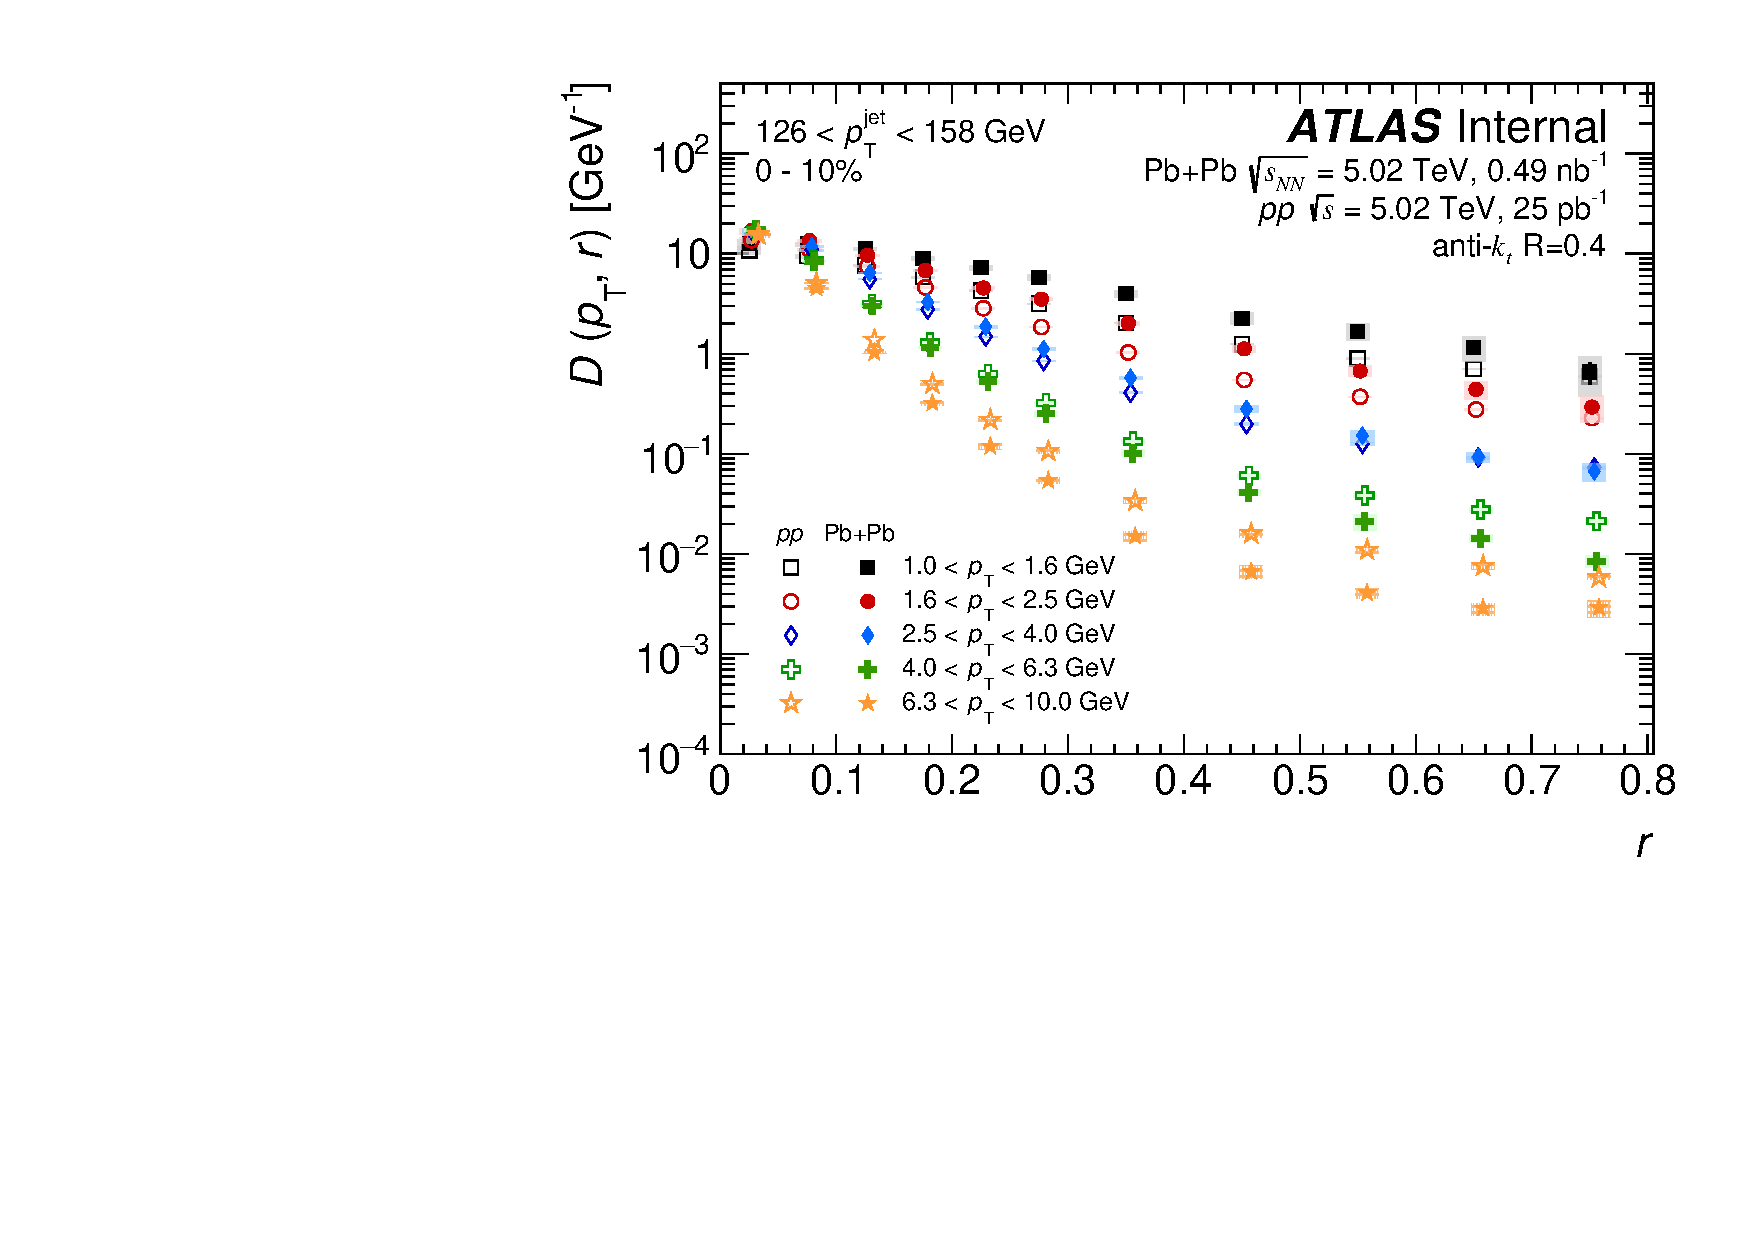
\includegraphics[width=0.5\textwidth]{figures/results/ChPS_final_dR_CONF_DpT_data_jet7_cent0.pdf} & 
%            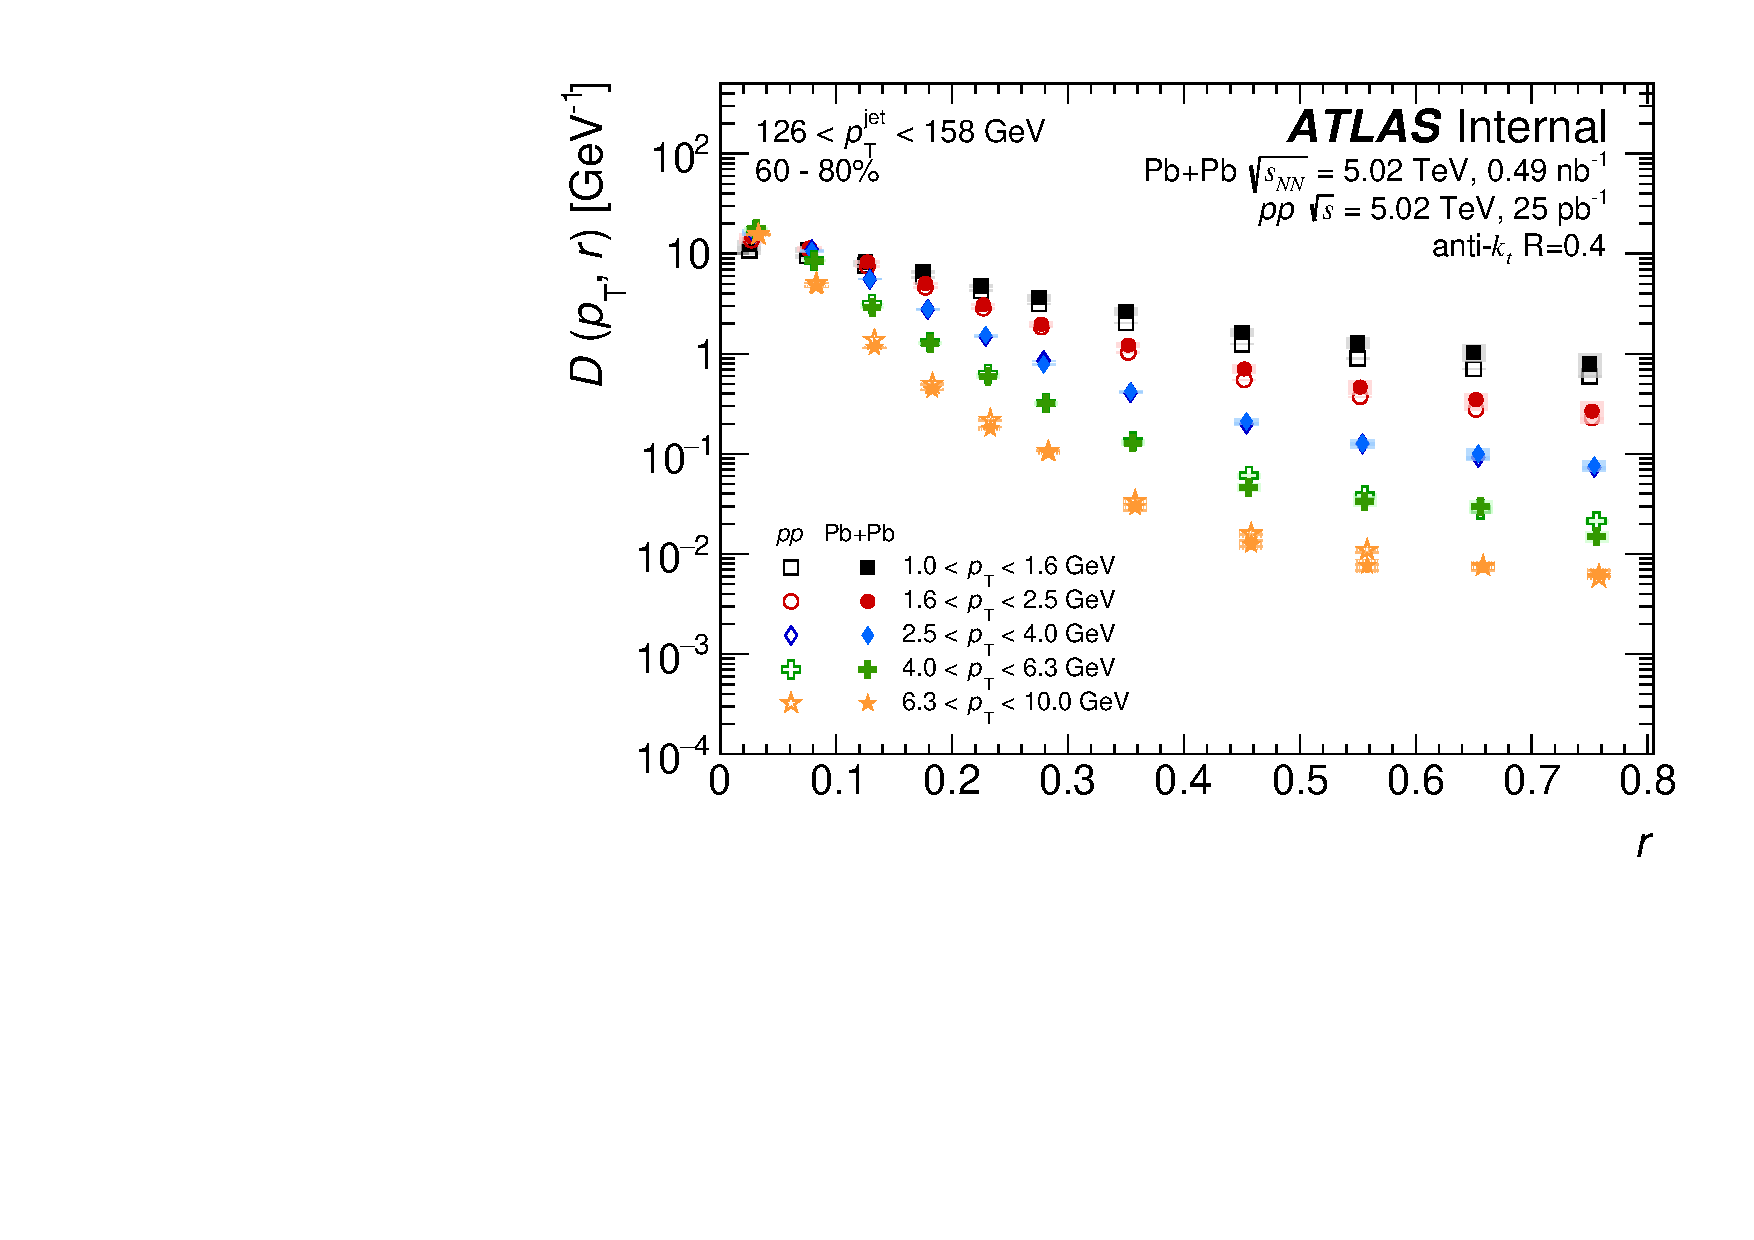
\includegraphics[width=0.5\textwidth]{figures/results/ChPS_final_dR_CONF_DpT_data_jet7_cent5.pdf} \\
%            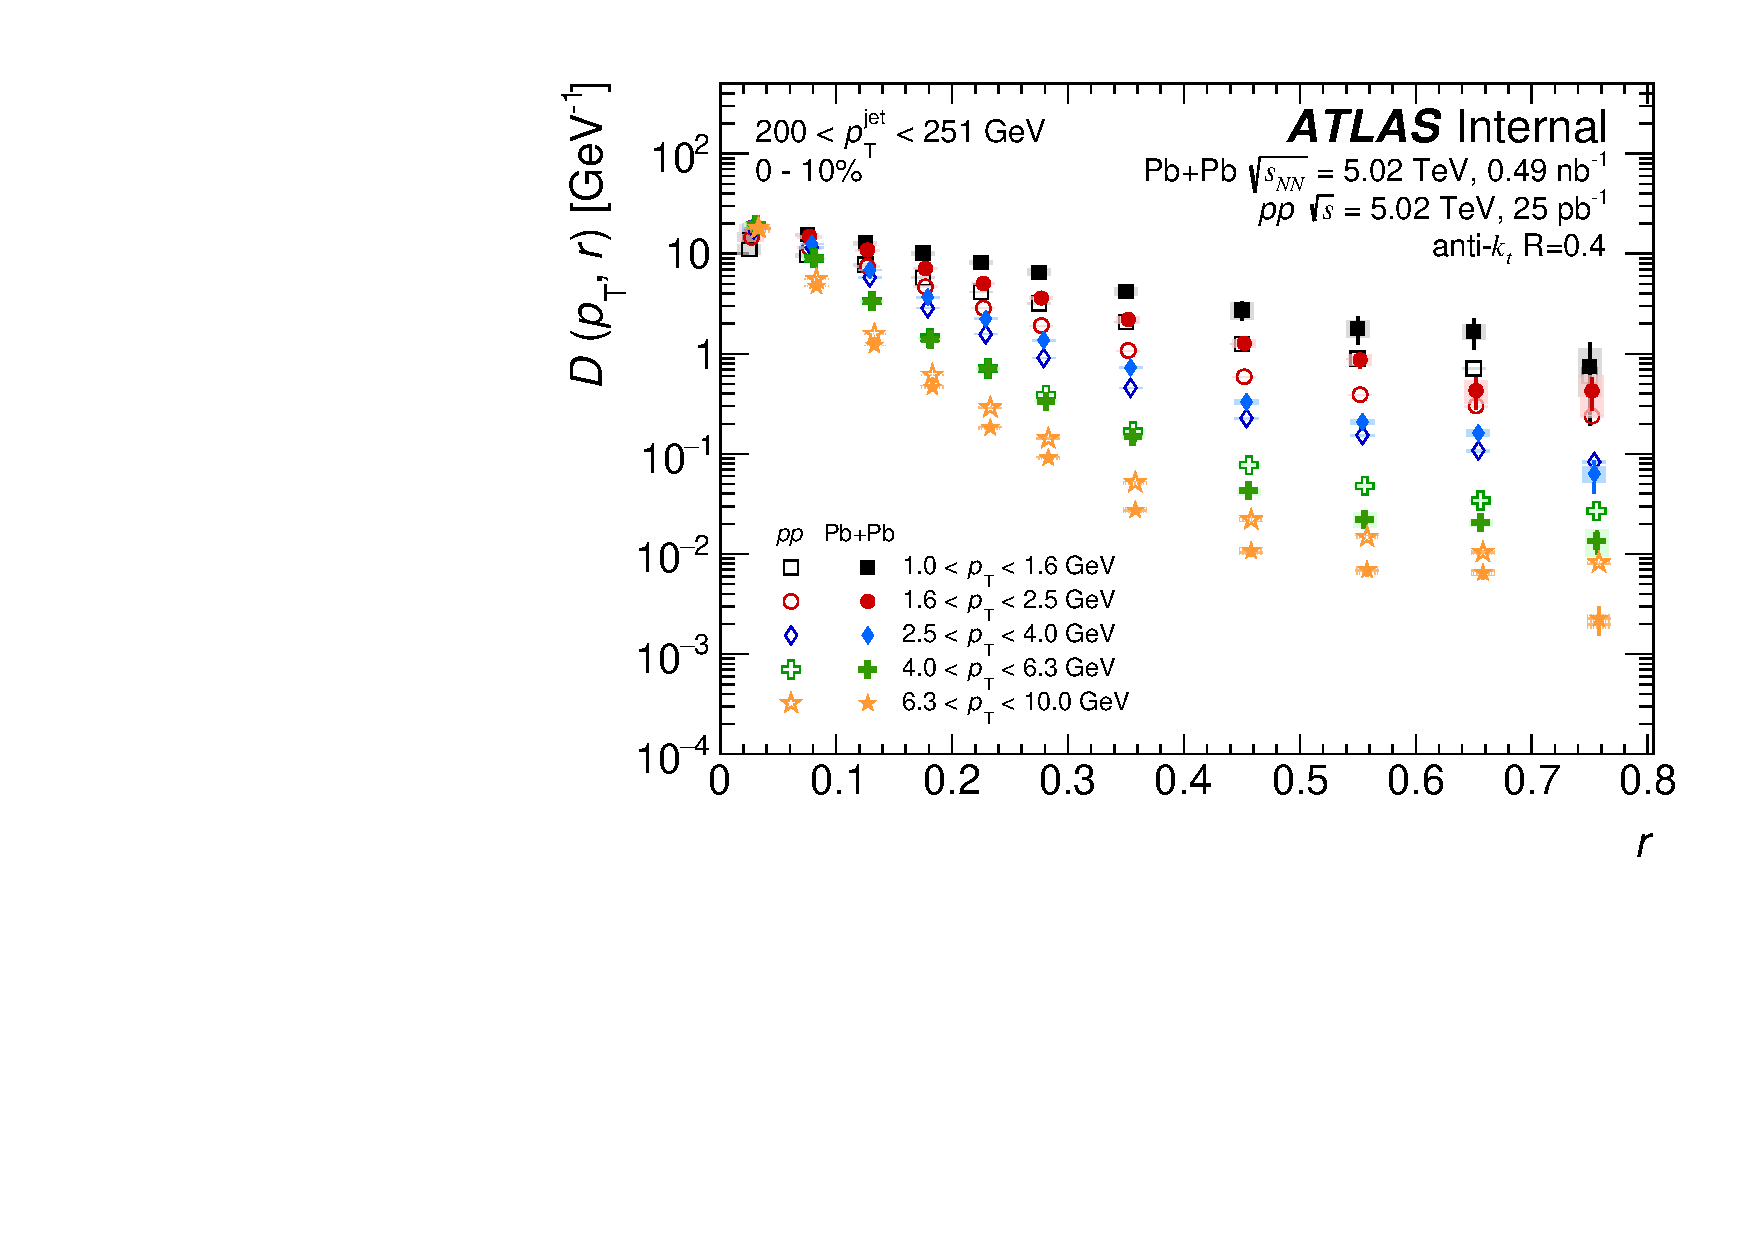
\includegraphics[width=0.5\textwidth]{figures/results/ChPS_final_dR_CONF_DpT_data_jet9_cent0.pdf} & 
%            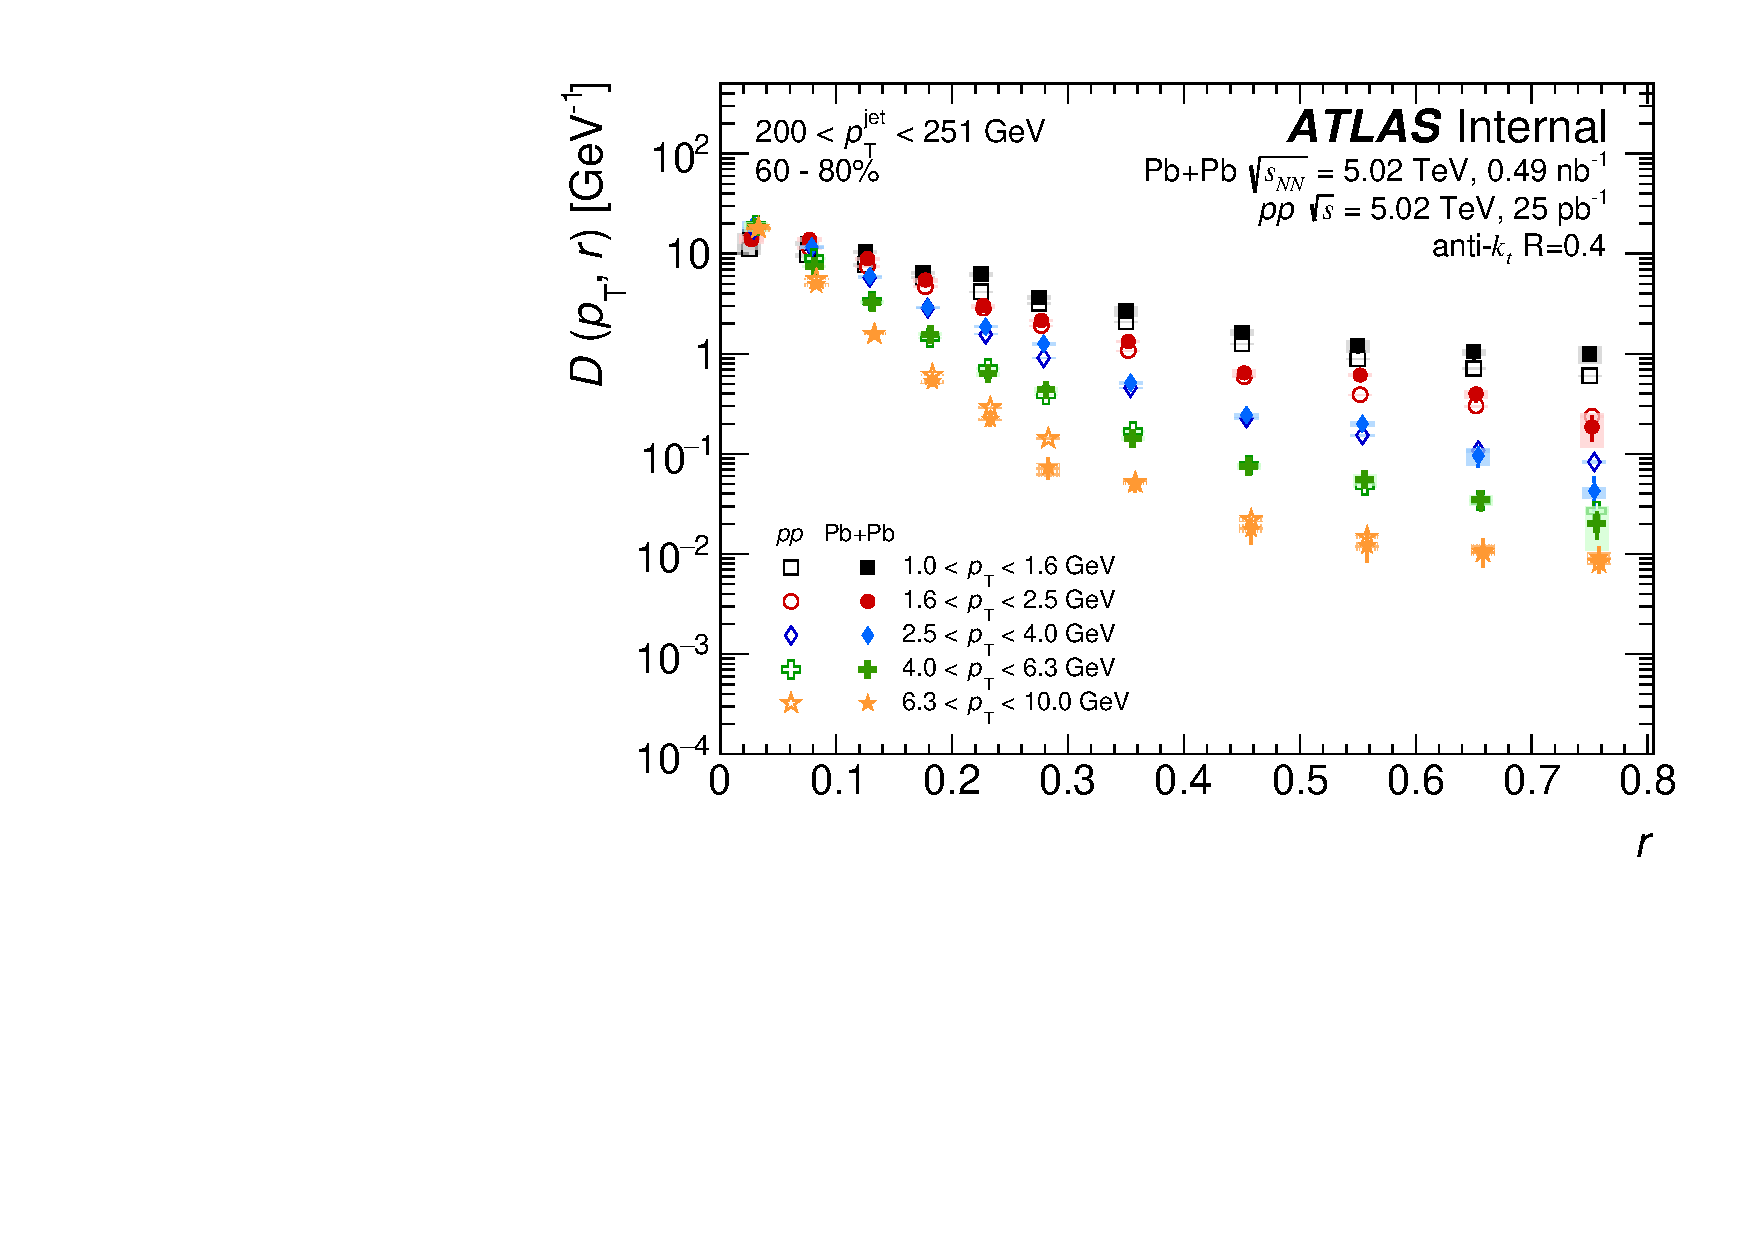
\includegraphics[width=0.5\textwidth]{figures/results/ChPS_final_dR_CONF_DpT_data_jet9_cent5.pdf} \\
%      \end{tabular}
%      }
%\caption{Closed symbols show \Dptr\ distributions in 0--10\% (left) and 60--80\% (right) \pbpb\ as a function of angular distance $r$ for \ptjet\ of 126 to 158~\GeV\ (top) and of 200 to 251~\GeV\ (bottom) for four \pt\ selections. Open symbols show \Dptr\ distributions in \pp\ collisions.  The vertical bars on the data points indicate statistical uncertainties while the shaded boxes indicate systematic uncertainties. There are no uncertainties on the \rvar\ values, the finite widths of the shaded boxes are purely aesthetic.}
%\label{fig:dptr}
%\end{figure}

\begin{figure}[h]
\centerline{
            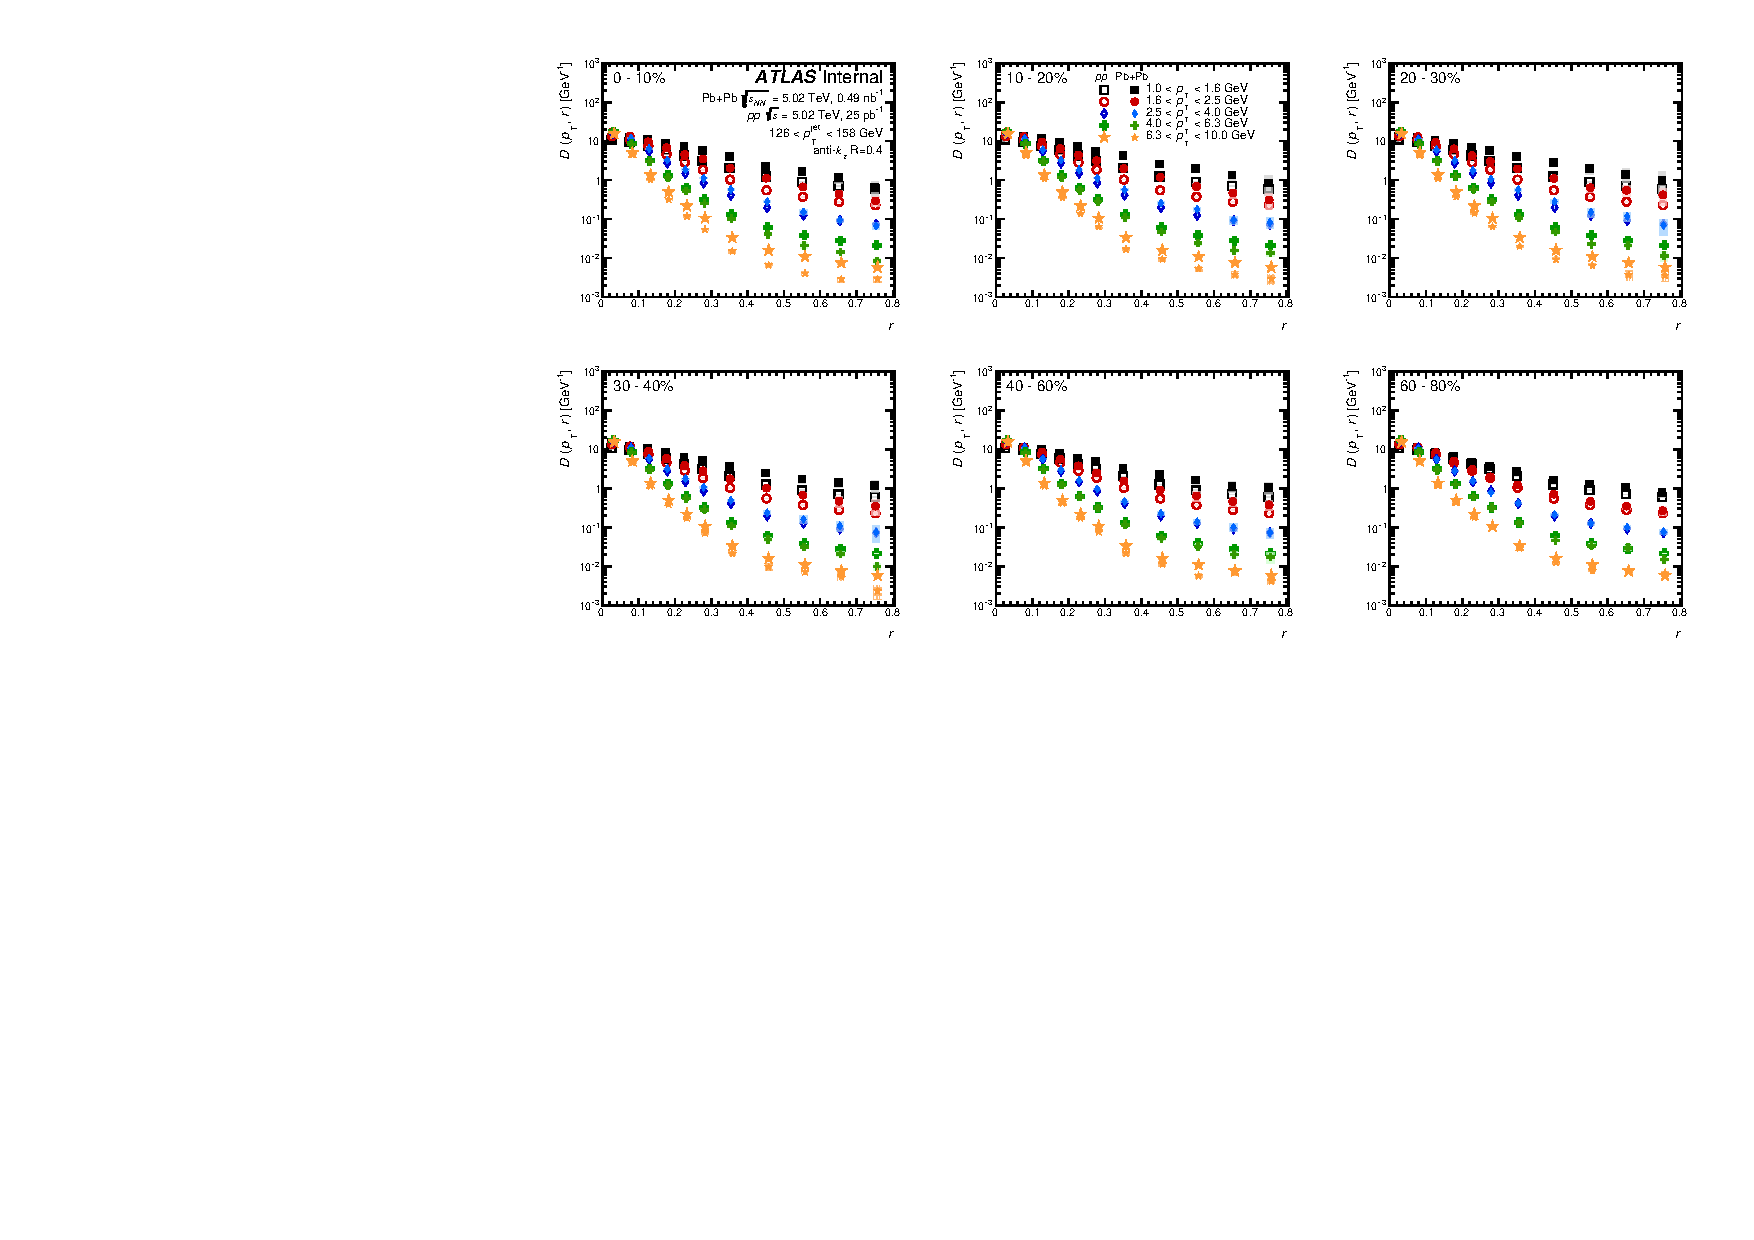
\includegraphics[width=1\textwidth]{figures/results/yChPS_final_dR_CONF_DpT_data_jet7.pdf} 
      }
\caption{The \Dptr\ distributions in \pp\ (open symbols) and \pbpb\ (closed symbols) as a function of angular distance $r$ for \ptjet\ of 126 to 158~\GeV. The different curves are different track \pt\ ranges, and the different panels are different centrality selections. The vertical bars on the data points indicate statistical uncertainties while the shaded boxes indicate systematic uncertainties. There are no uncertainties on the \rvar\ values, the finite widths of the shaded boxes are purely aesthetic.}
\label{fig:dptr}
\end{figure}


%The ratios of \Dptr\ distributions measured in \pbpb\ collisions to those measured in \pp\ collisions, \RDptr, are evaluated to quantify the modifications in \PbPb\ compared to \pp\ collisions.
Ratios of the \Dptr\ distributions in \pbpb\ to those measured in \pp\ are presented in Figure~\ref{fig:rdptr} as a function of $r$ for different \pt\ selections. In 0--10\% central collisions, 
\RDptr\ is above unity at all \rvar\ for charged-particles with \pT less than 4~\GeV.
For these particles, 
\RDptr\  grows with increasing \rvar\ for \rvar\ $ < 0.3$ is approximately constant for \mbox{$ 0.3 <$ \rvar\ $< 0.6 $}, and decreases for \mbox{$0.6 < \rvar < 0.8$}.  For $\pt > 4.0$ \GeV, \RDptr\ is below unity and decreases with increasing \rvar\ for $r < 0.3$ and is approximately constant for \mbox{$ 0.3 <$ \rvar\ $< 0.8 $}.  The observed behavior inside the jet ($r < 0.4$) agrees with the measurement of the inclusive jet fragmentation functions~\cite{Aaboud:2017eww, PhysRevC.98.024908}, where yields of the low-$\pT$ fragments are observed to be enhanced and yields of charged particles with intermediate \pT\ are suppressed in \PbPb\ collisions compared to those in \pp\ collisions. 
For peripheral collisions, \RDptr\ has no significant \rvar\ dependence and the distributions do not significantly deviate from unity. % for charged particles with  $\pt <$~4.0~\GeV; for higher \pt\ particles \RDptr\ decreases with increasing \rvar. 
The measured dependence of \RDptr\ suggests that the energy lost by jets through the jet quenching process is being transferred to particles with $\pt <$~4.0~\GeV\ with larger radial distances. This is qualitatively consistent with theoretical calculations \mbox{\cite{Qin:2015srf,Blaizot:2014ula}}.


The centrality dependence of \RDptr\ is presented in Figure~\ref{fig:centdep} where the \RDptr\ for two \pt\ selections: 1.6--2.5~\GeV\ and \mbox{6.3--10.0~\GeV}, and 
all centrality intervals are shown. The magnitude of these modifications decreases for more peripheral collisions and \RDptr\ goes towards unity in 60--80\% central collisions for both \pt\ ranges, across the entire $ r < 0.8$ range under investigation. This observation is in agreement with previous measurements of jet fragmentation functions \cite{Chatrchyan:2014ava, Sirunyan:2018jqr, Aaboud:2017bzv, PhysRevC.98.024908}.
 

\begin{figure}[h]
\centerline{
         \begin{tabular}{cc}
            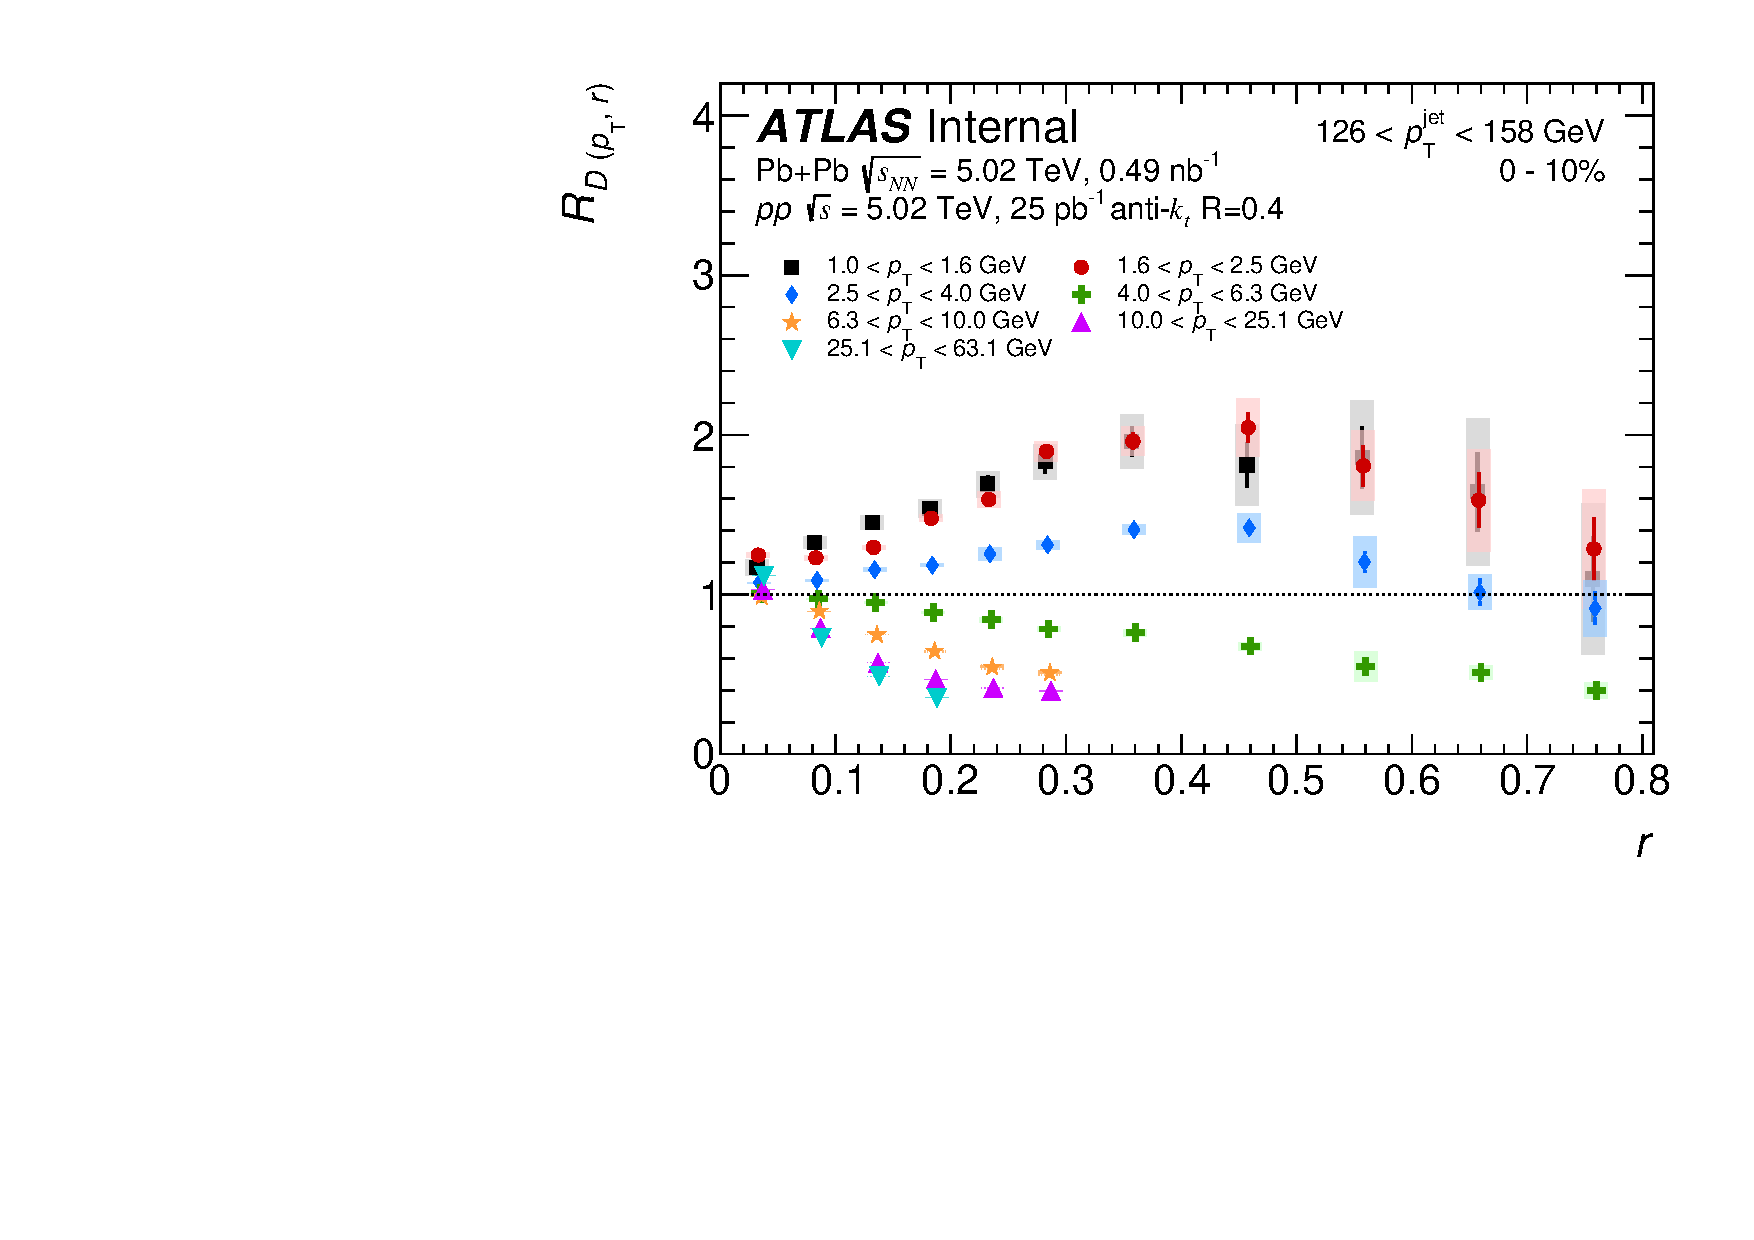
\includegraphics[width=0.5\textwidth]{figures/results/RDpT_final_ratio_dR_CONF_data_jet7_cent0.pdf} & 
            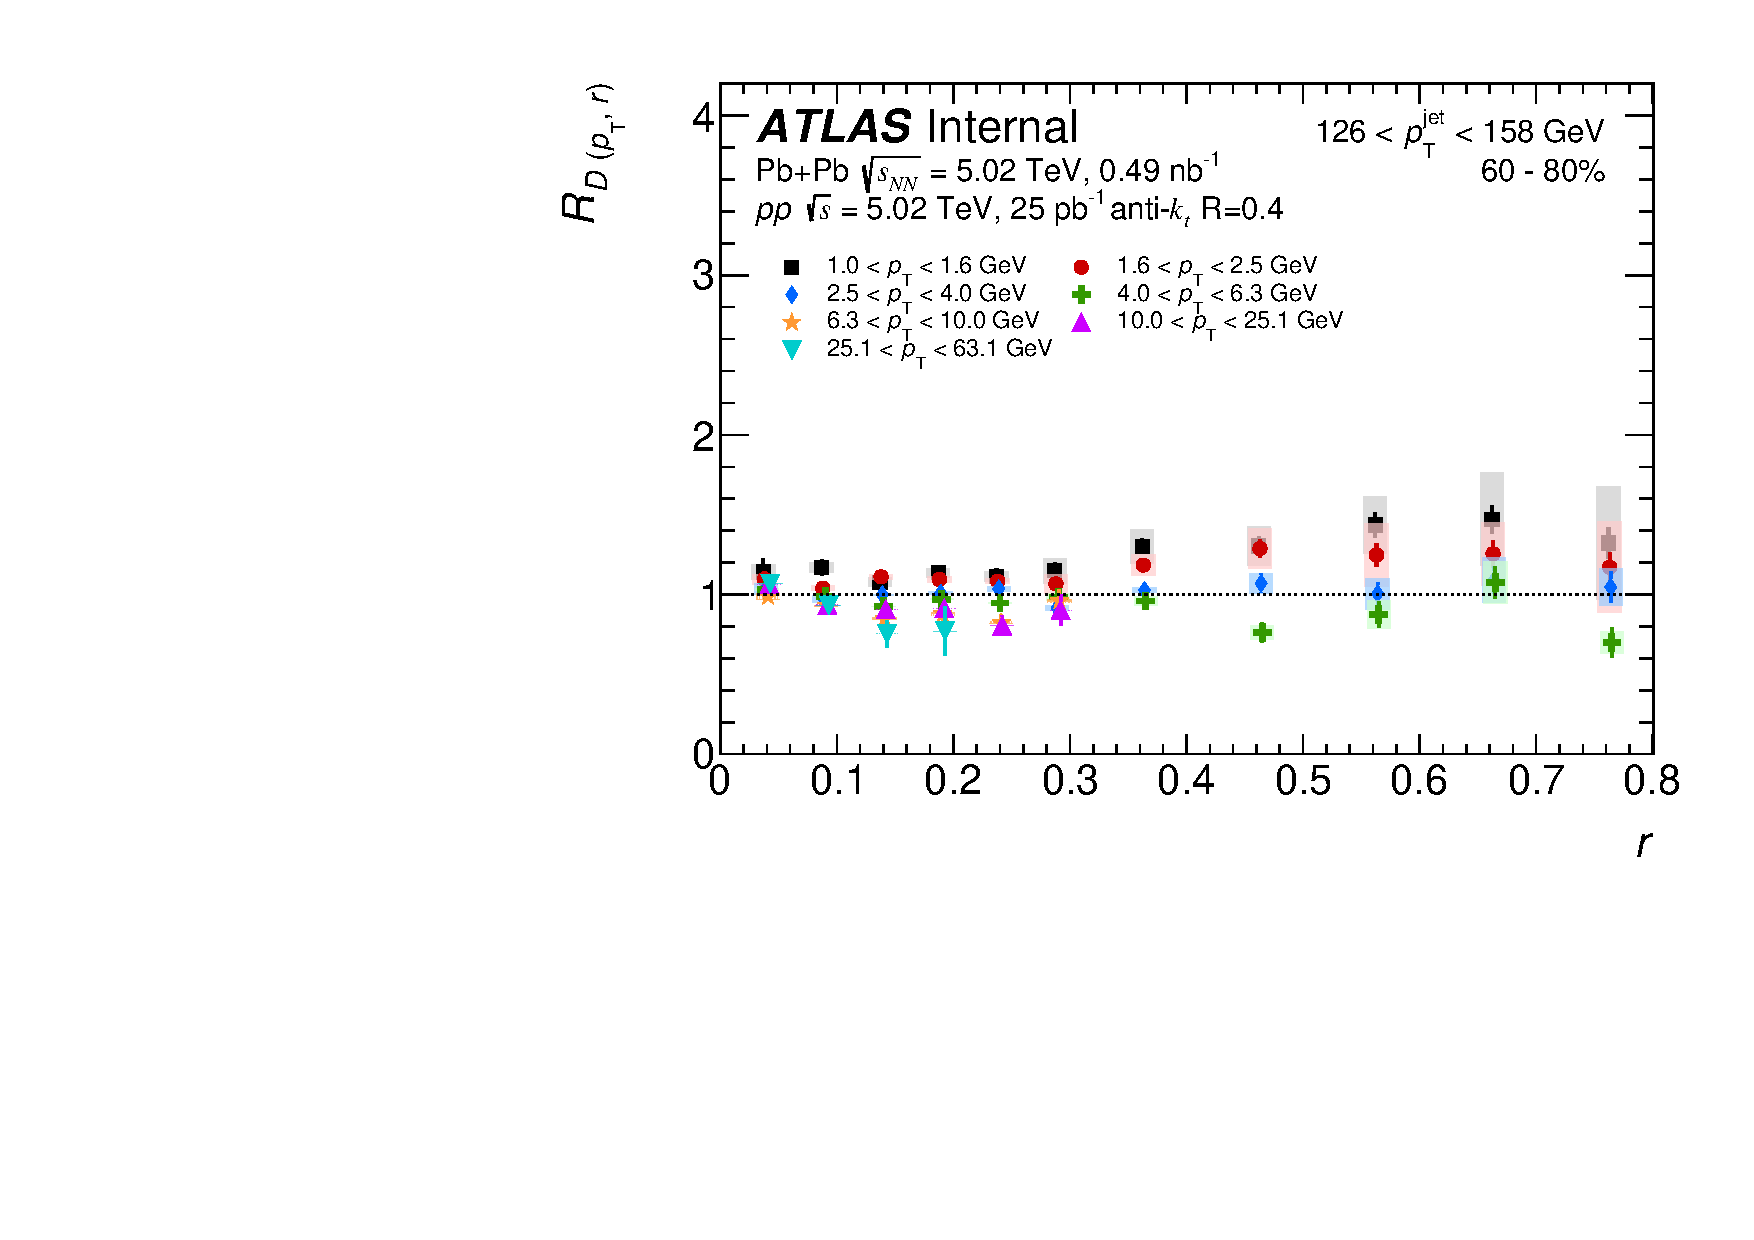
\includegraphics[width=0.5\textwidth]{figures/results/RDpT_final_ratio_dR_CONF_data_jet7_cent5.pdf} \\
            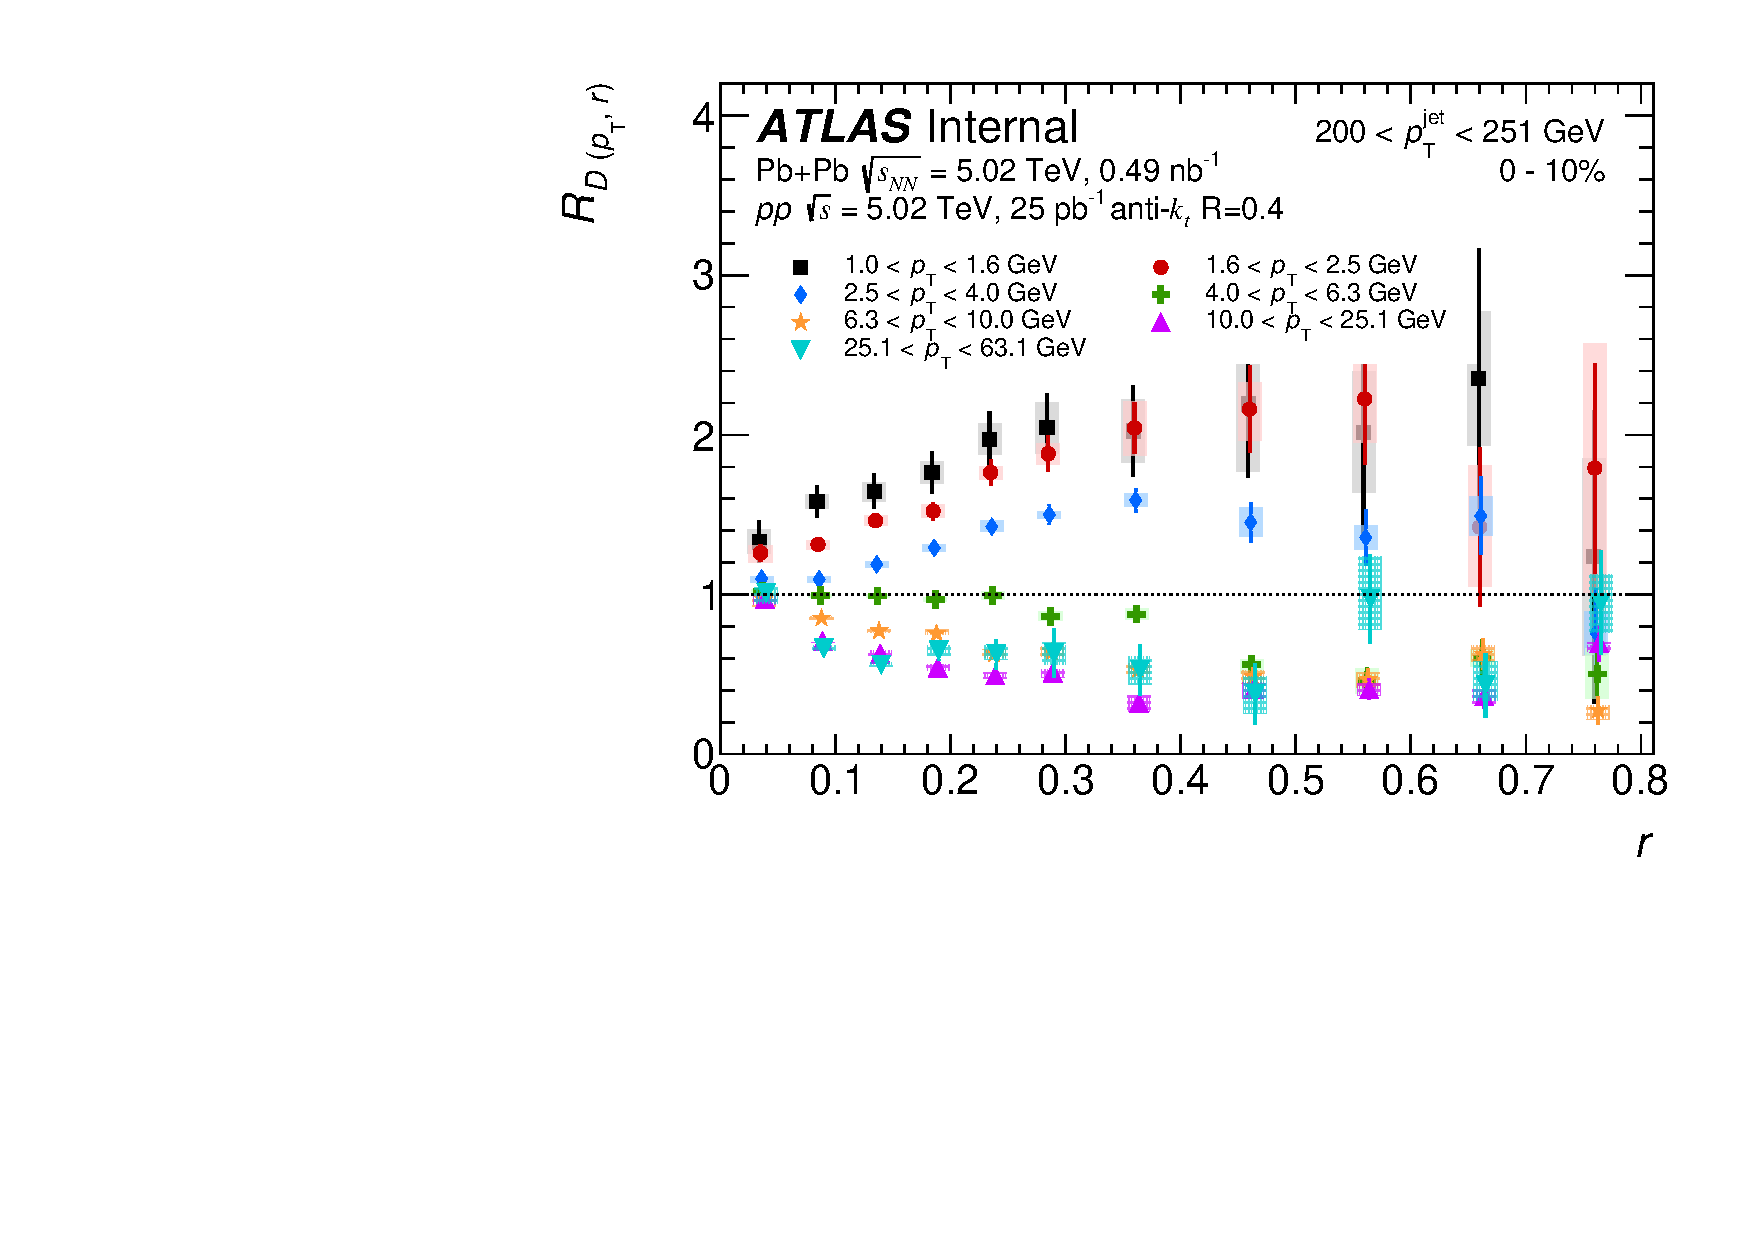
\includegraphics[width=0.5\textwidth]{figures/results/RDpT_final_ratio_dR_CONF_data_jet9_cent0.pdf} & 
            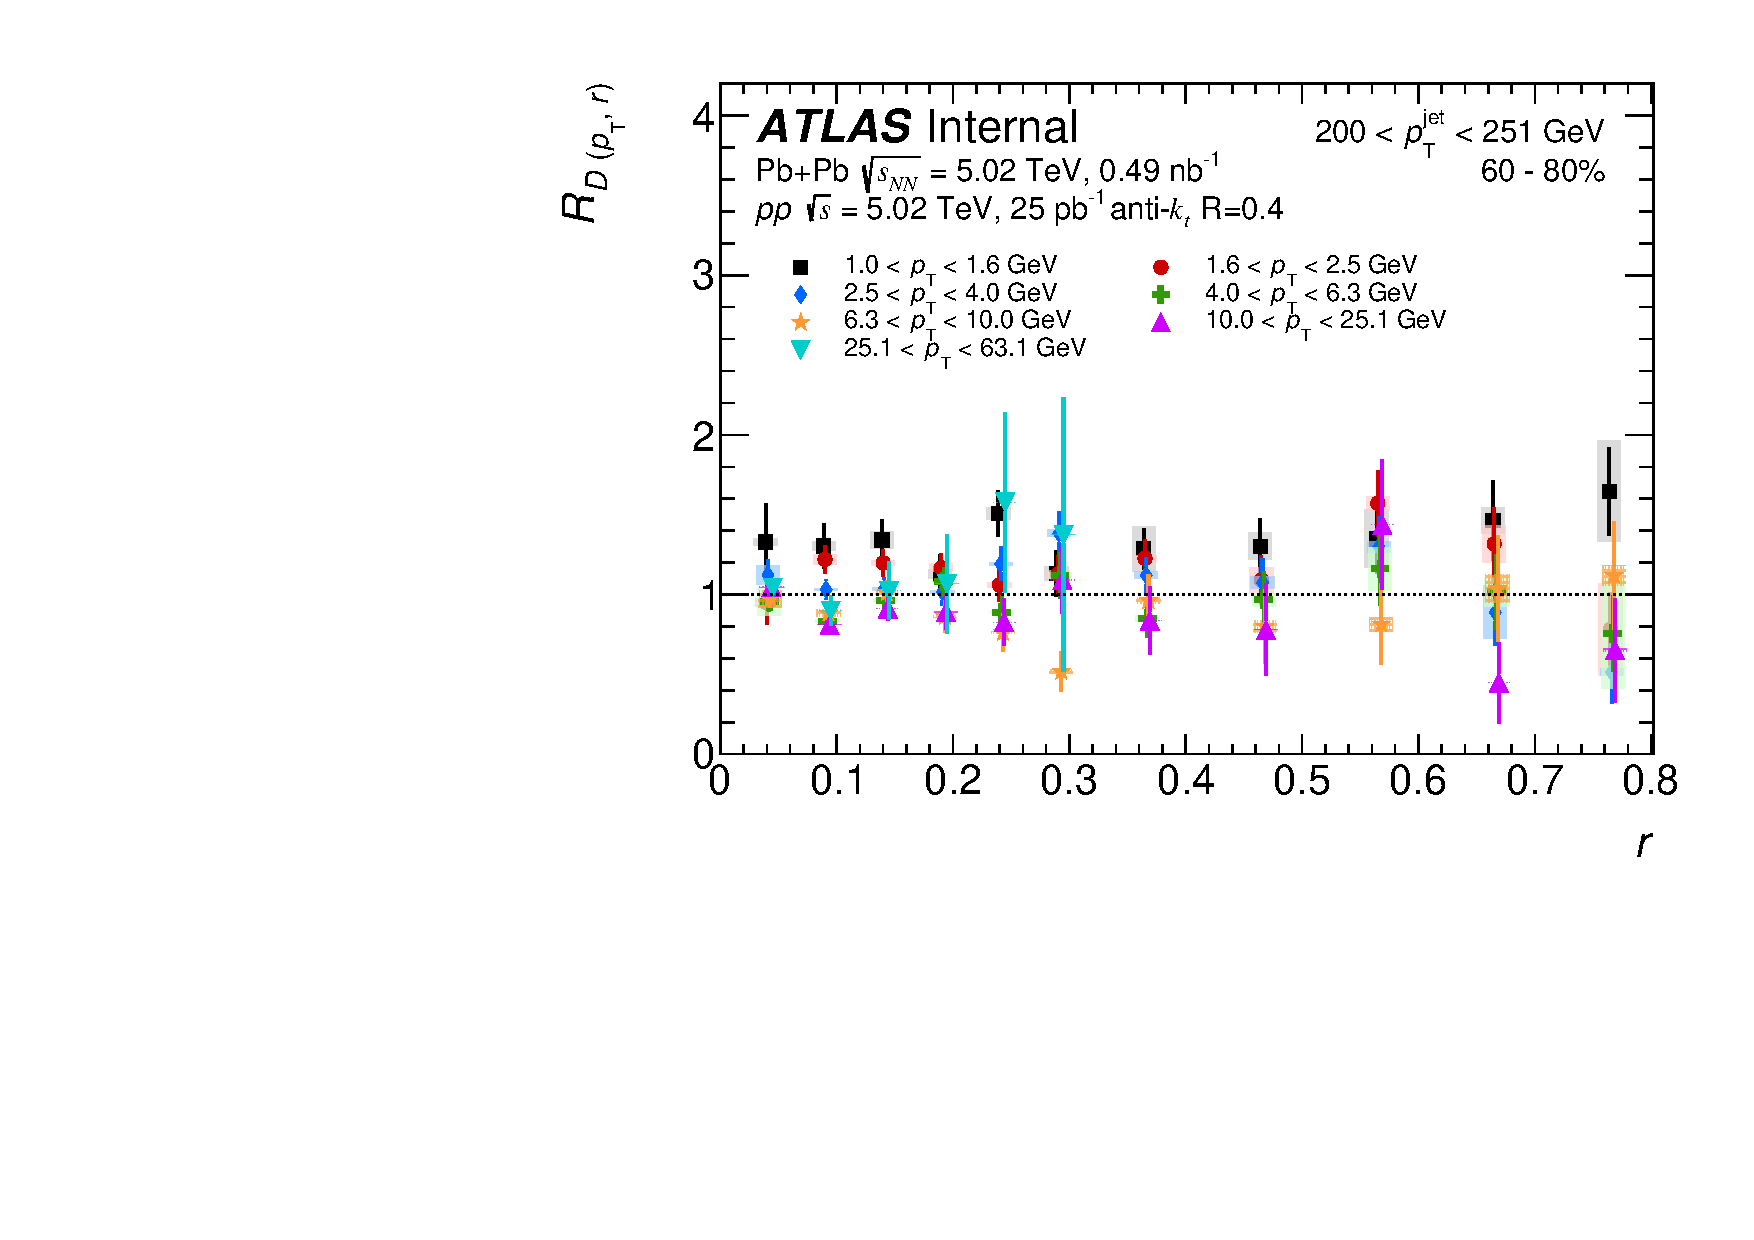
\includegraphics[width=0.5\textwidth]{figures/results/RDpT_final_ratio_dR_CONF_data_jet9_cent5.pdf} \\
      \end{tabular}
      }
\caption{Ratios of \Dptr\ distributions in 0--10\% (left) and 60--80\% (right) \PbPb\ collisions to \pp\ collisions as a function of angular distance $r$ for \ptjet\ of 126 to 158~\GeV\ (top) and of 200 to 251~\GeV\ (bottom) for six \pt\ selections.  The vertical bars on the data points indicate statistical uncertainties while the shaded boxes indicate systematic uncertainties. There are no uncertainties on the \rvar\ values, the finite widths of the shaded boxes are purely aesthetic.}
\label{fig:rdptr}
\end{figure}

\begin{figure}[h]
\centerline{
         \begin{tabular}{cc}
            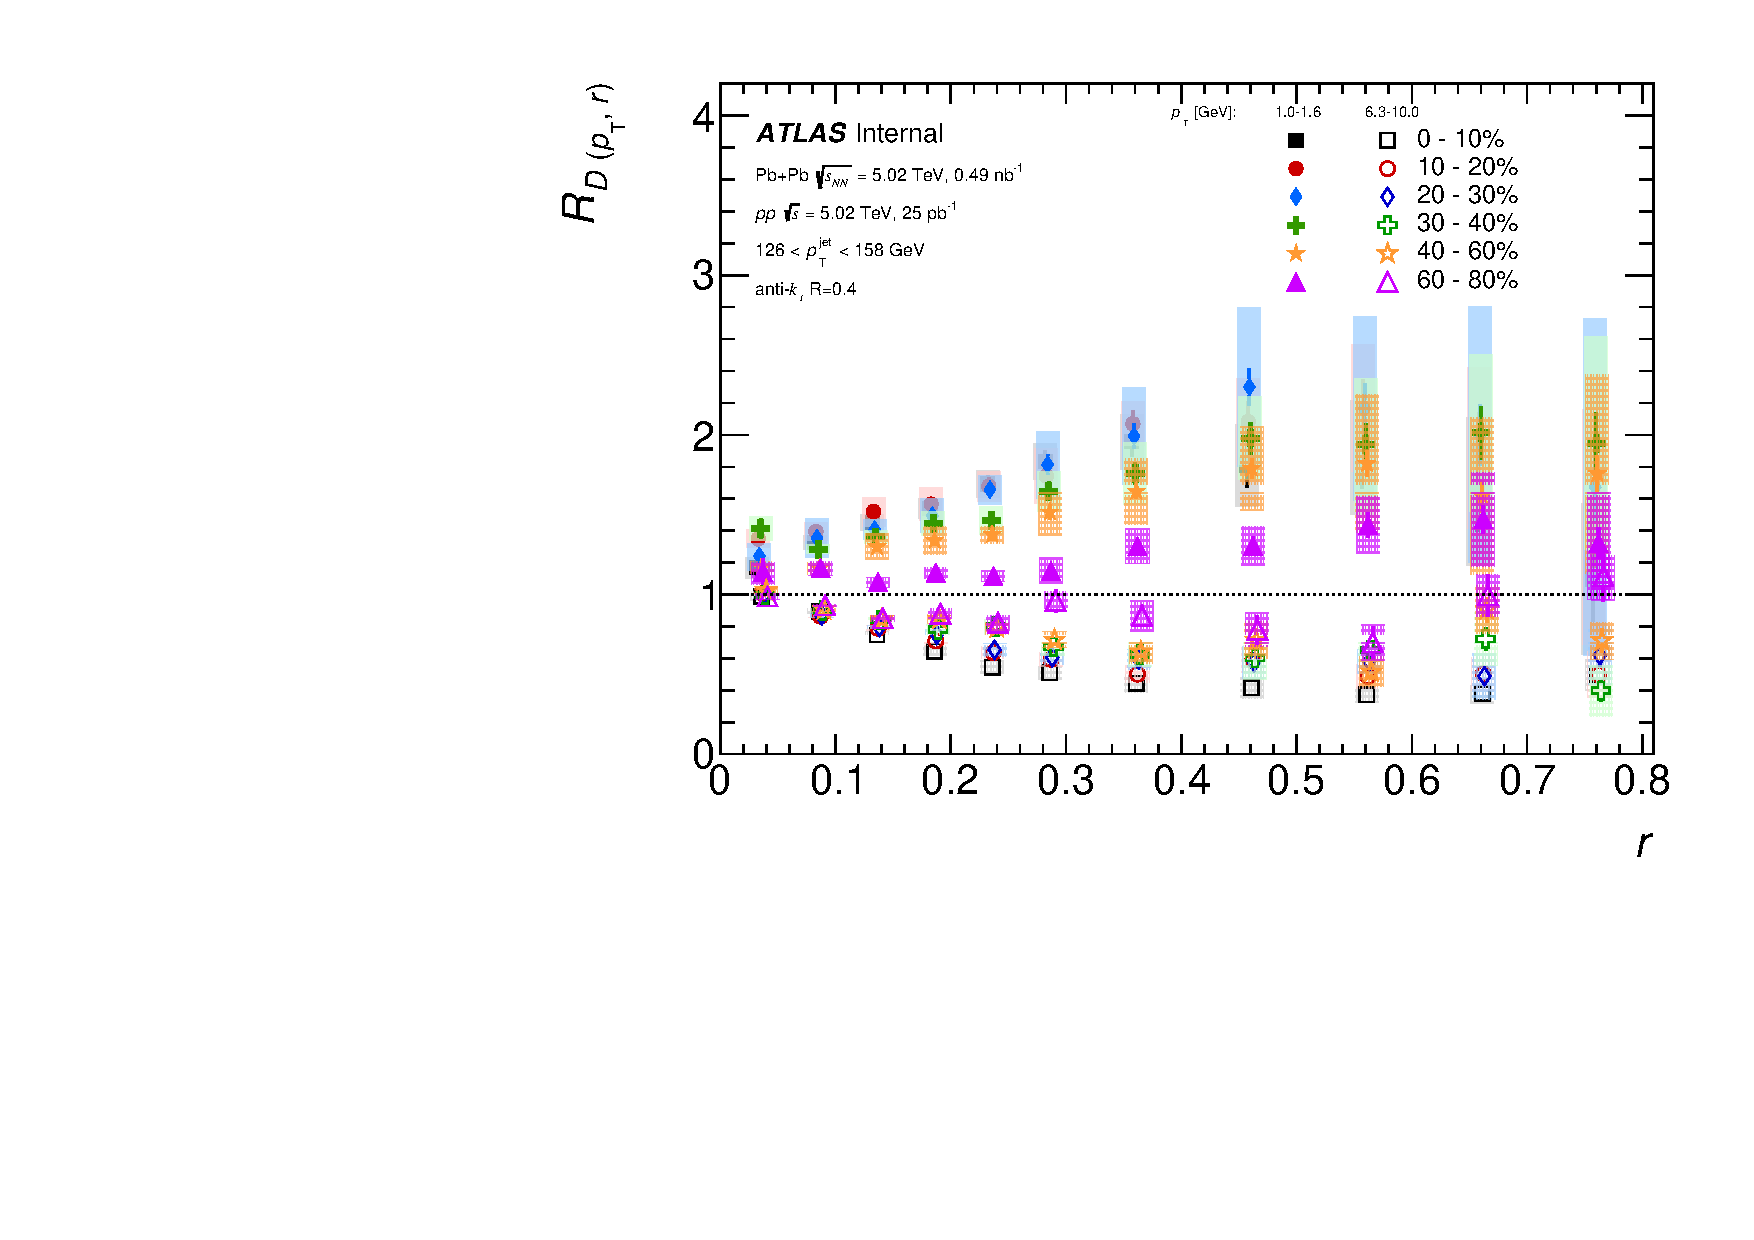
\includegraphics[width=0.5\textwidth]{figures/results/RDpT_final_dR_CONF_data_cent_trk2_6_jet7.pdf} & 
            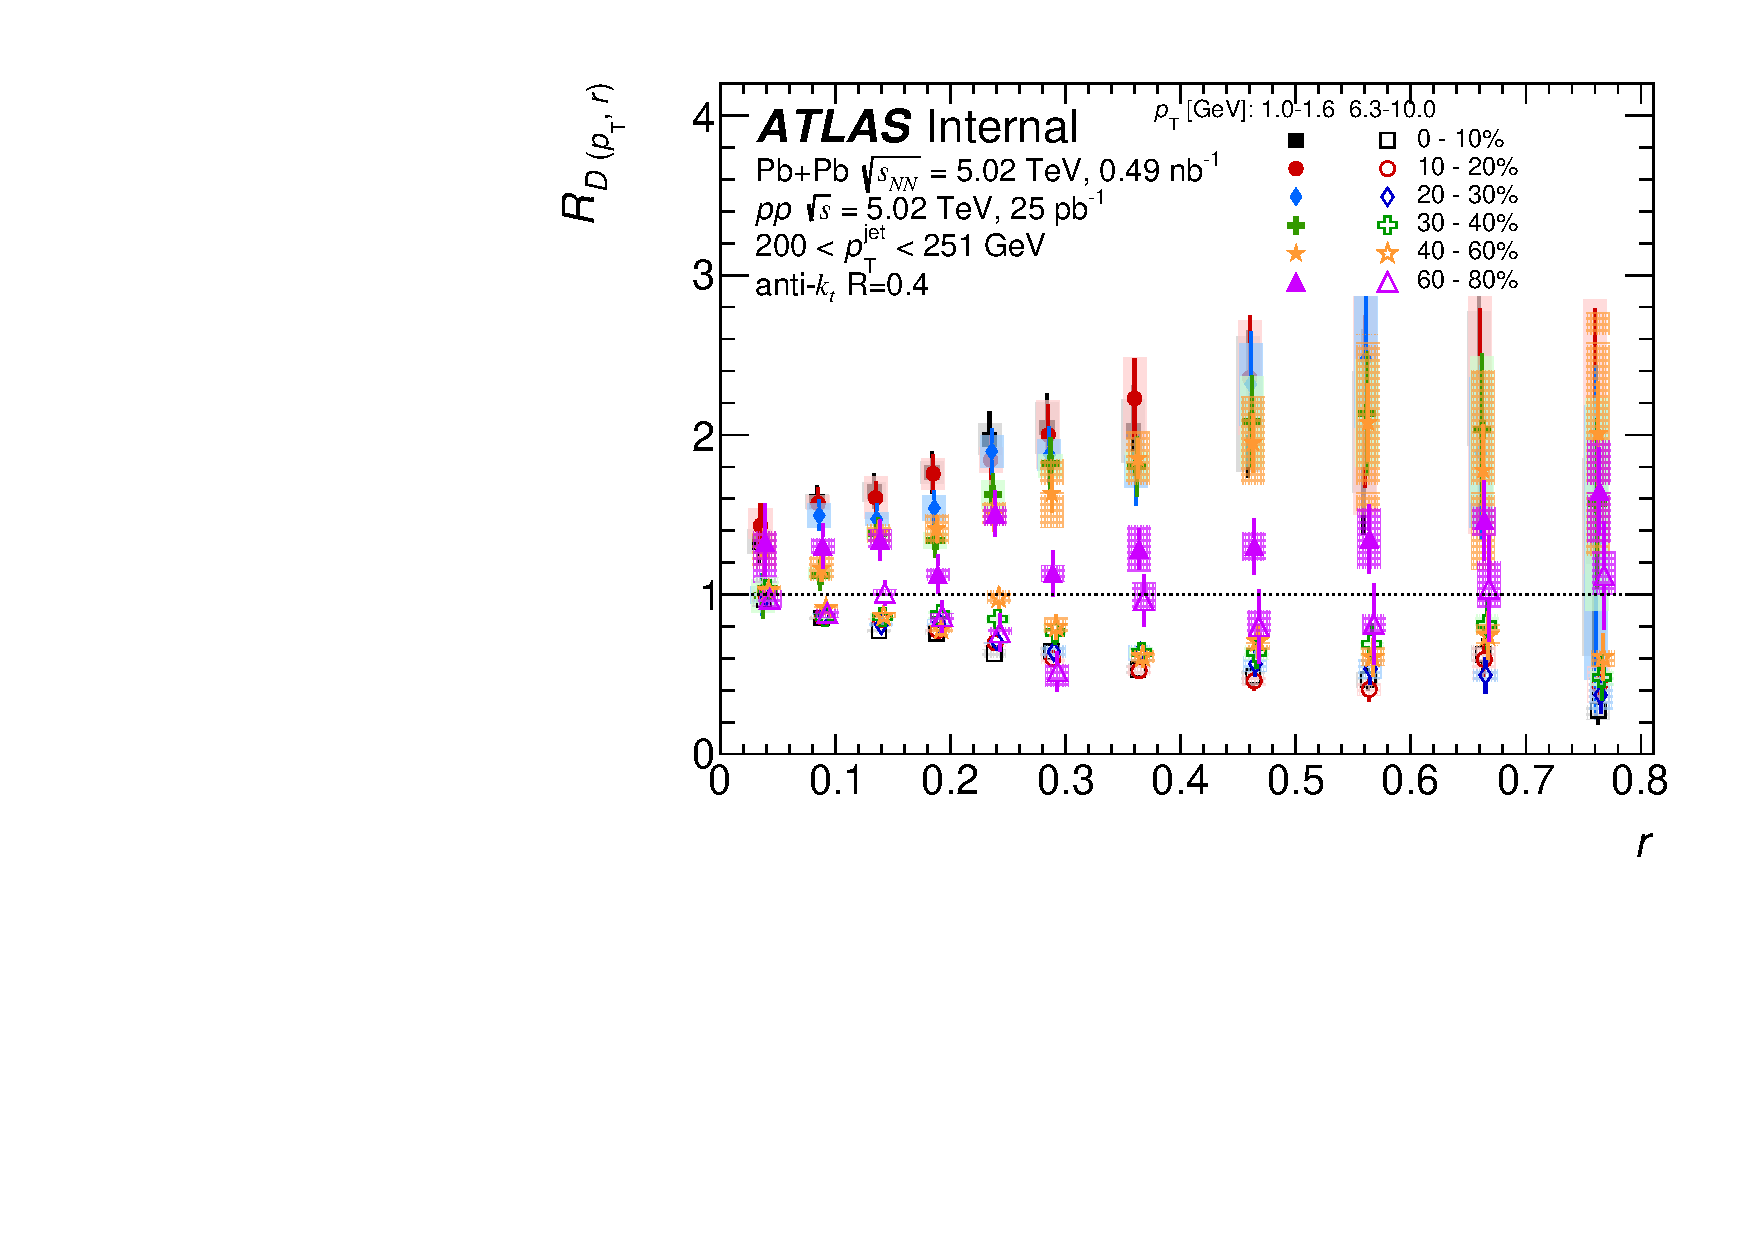
\includegraphics[width=0.5\textwidth]{figures/results/RDpT_final_dR_CONF_data_cent_trk2_6_jet9.pdf} \\
      \end{tabular}
      }
\caption{Ratios of \Dptr\ distributions for \ptjet\ of 126 to 158~\GeV\ (left) and of 200 to 251~\GeV\ (right) in \PbPb\ collisions to \pp\ collisions as a function of angular distance $r$ for two \pt\ selections and six centrality intervals (\pt\ selections are shown by closed and open symbols). The vertical bars on the data points indicate statistical uncertainties while the shaded boxes indicate systematic uncertainties. There are no uncertainties on the \rvar\ values, the finite widths of the shaded boxes are purely aesthetic.}
\label{fig:centdep}
\end{figure}

\begin{figure}[ht]
\centerline{
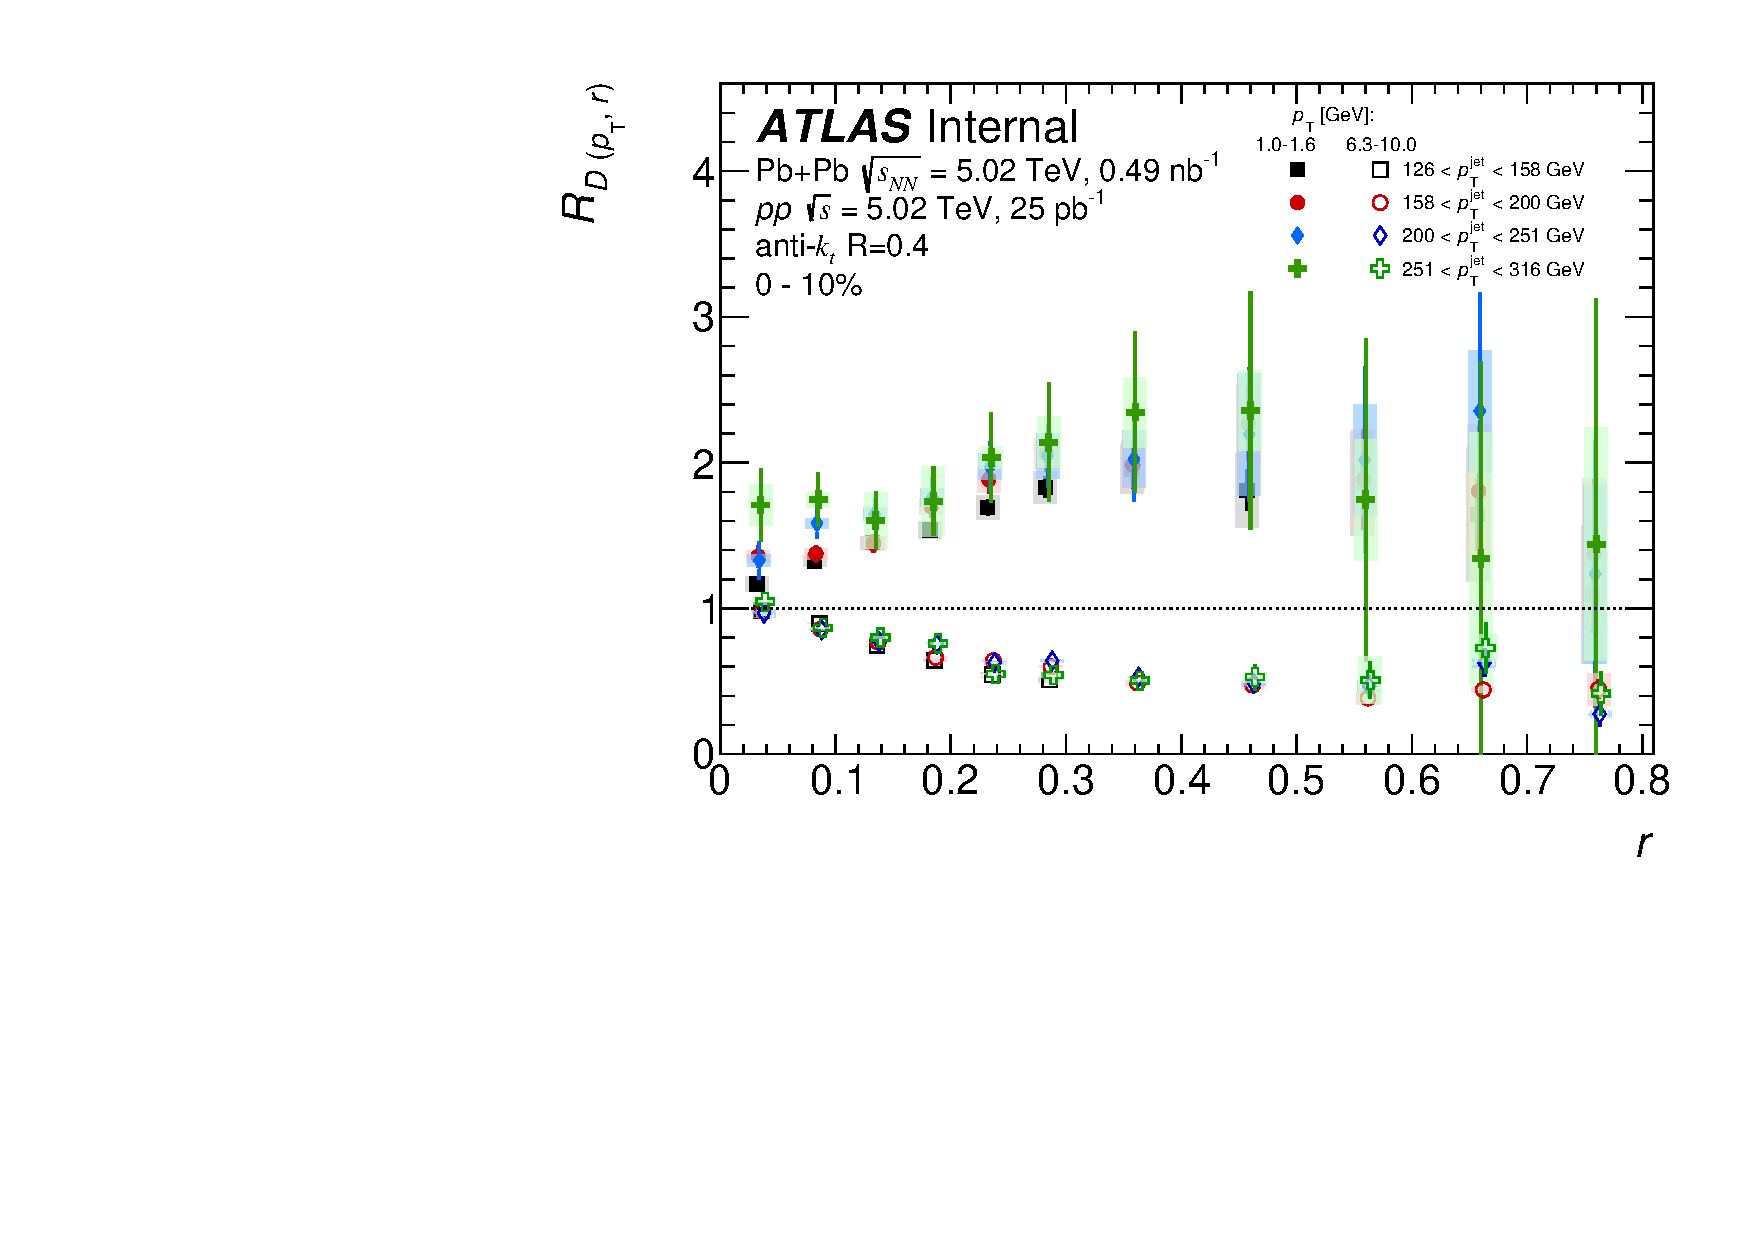
\includegraphics[width=0.8\textwidth]{figures/results/RDpT_final_ratio_dR_CONF_data_trk2_6_cent0.pdf} 
}
\caption{\RDptr\ as a function of \rvar\ for 0--10\% collisions for charged particles with 1.6~$< \pt <$~2.5~\GeV\
(closed symbols) and 6.3~$< \pt <$10.0~\GeV\ (open symbols) for four \ptjet\ selections: 126--158~\GeV, 158--200~\GeV,
200--251~\GeV, and 251--316~\GeV. There are no uncertainties on the \rvar\ values, the finite widths of the shaded boxes are purely aesthetic.}
\label{fig:ptjetdep}
\end{figure}

The \ptjet\ dependence of \RDptr\ in 0--10\% central collisions is presented in Figure~\ref{fig:ptjetdep} where the \RDptr\ for two \pt selections: 1.0--1.6~\GeV\ and \mbox{6.3--10.0~\GeV}, and four \ptjet\ selections is shown. A statistically significant trend of increasing \RDptr\ with increasing \ptjet\ is observed for $0.1 < r < 0.25$ for low pt particles. This observation is in agreement with the previous measurement of jet fragmentation functions \cite{Chatrchyan:2014ava, Sirunyan:2018jqr, Aaboud:2017bzv, PhysRevC.98.024908} and may indicate the dependence of the response of the hot dense matter to the momentum of a jet passing through it. 
The higher-\pt\ charged particles have \RDptr\ values that decrease with increasing \rvar; no significant dependence on \ptjet\ is observed. 

The \pttrk\ dependence of \RDptr\ in 0--10\% central and 60--80\% peripheral collisions is presented in Figure~\ref{fig:pttrkdep} where the \RDptr\ at different distances from the jet axis: $0.00 < \rvar < 0.05$, $0.15 < \rvar < 0.20$, $0.30 < \rvar < 0.40$, $0.50 < \rvar < 0.60$, for $126 < \ptjet < 158$ GeV and $200 < \ptjet < 251$ GeV is shown. It can be seen that there is an enhancement in the number of particles in the jet core for all \pt, and that the depletion only happens for $\rvar > 0.05$. The enhancement is larger for higher \ptjet, and persists even for peripheral collisions. This observation is also in agreement with the previous measurement of jet fragmentation functions \cite{Chatrchyan:2014ava, Sirunyan:2018jqr, Aaboud:2017bzv, PhysRevC.98.024908} 

\begin{figure}
\centering{
\begin{tabular}{cc}
	 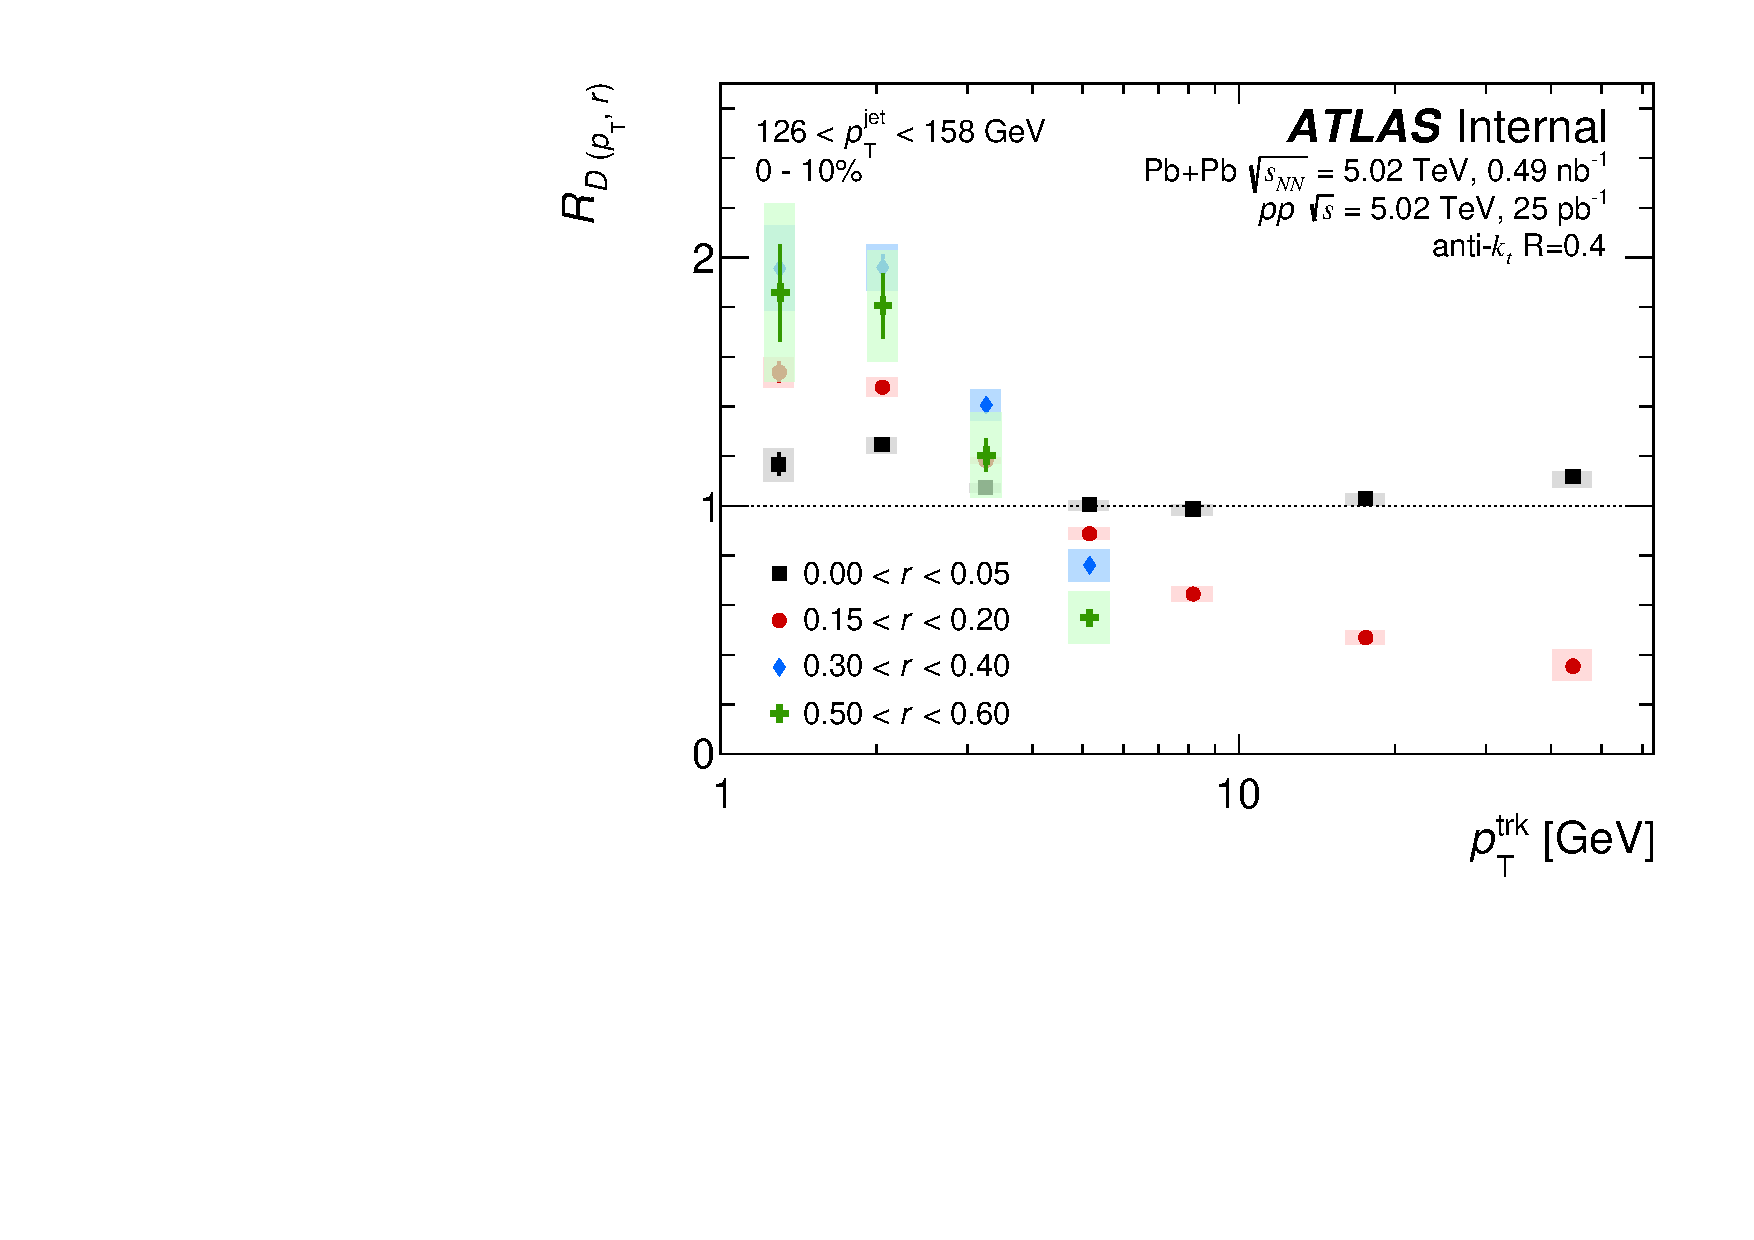
\includegraphics[width=0.45\textwidth]{results/RDpT_final_ratio_dR_CONF_data_trkpT_jet7_cent0} &
	 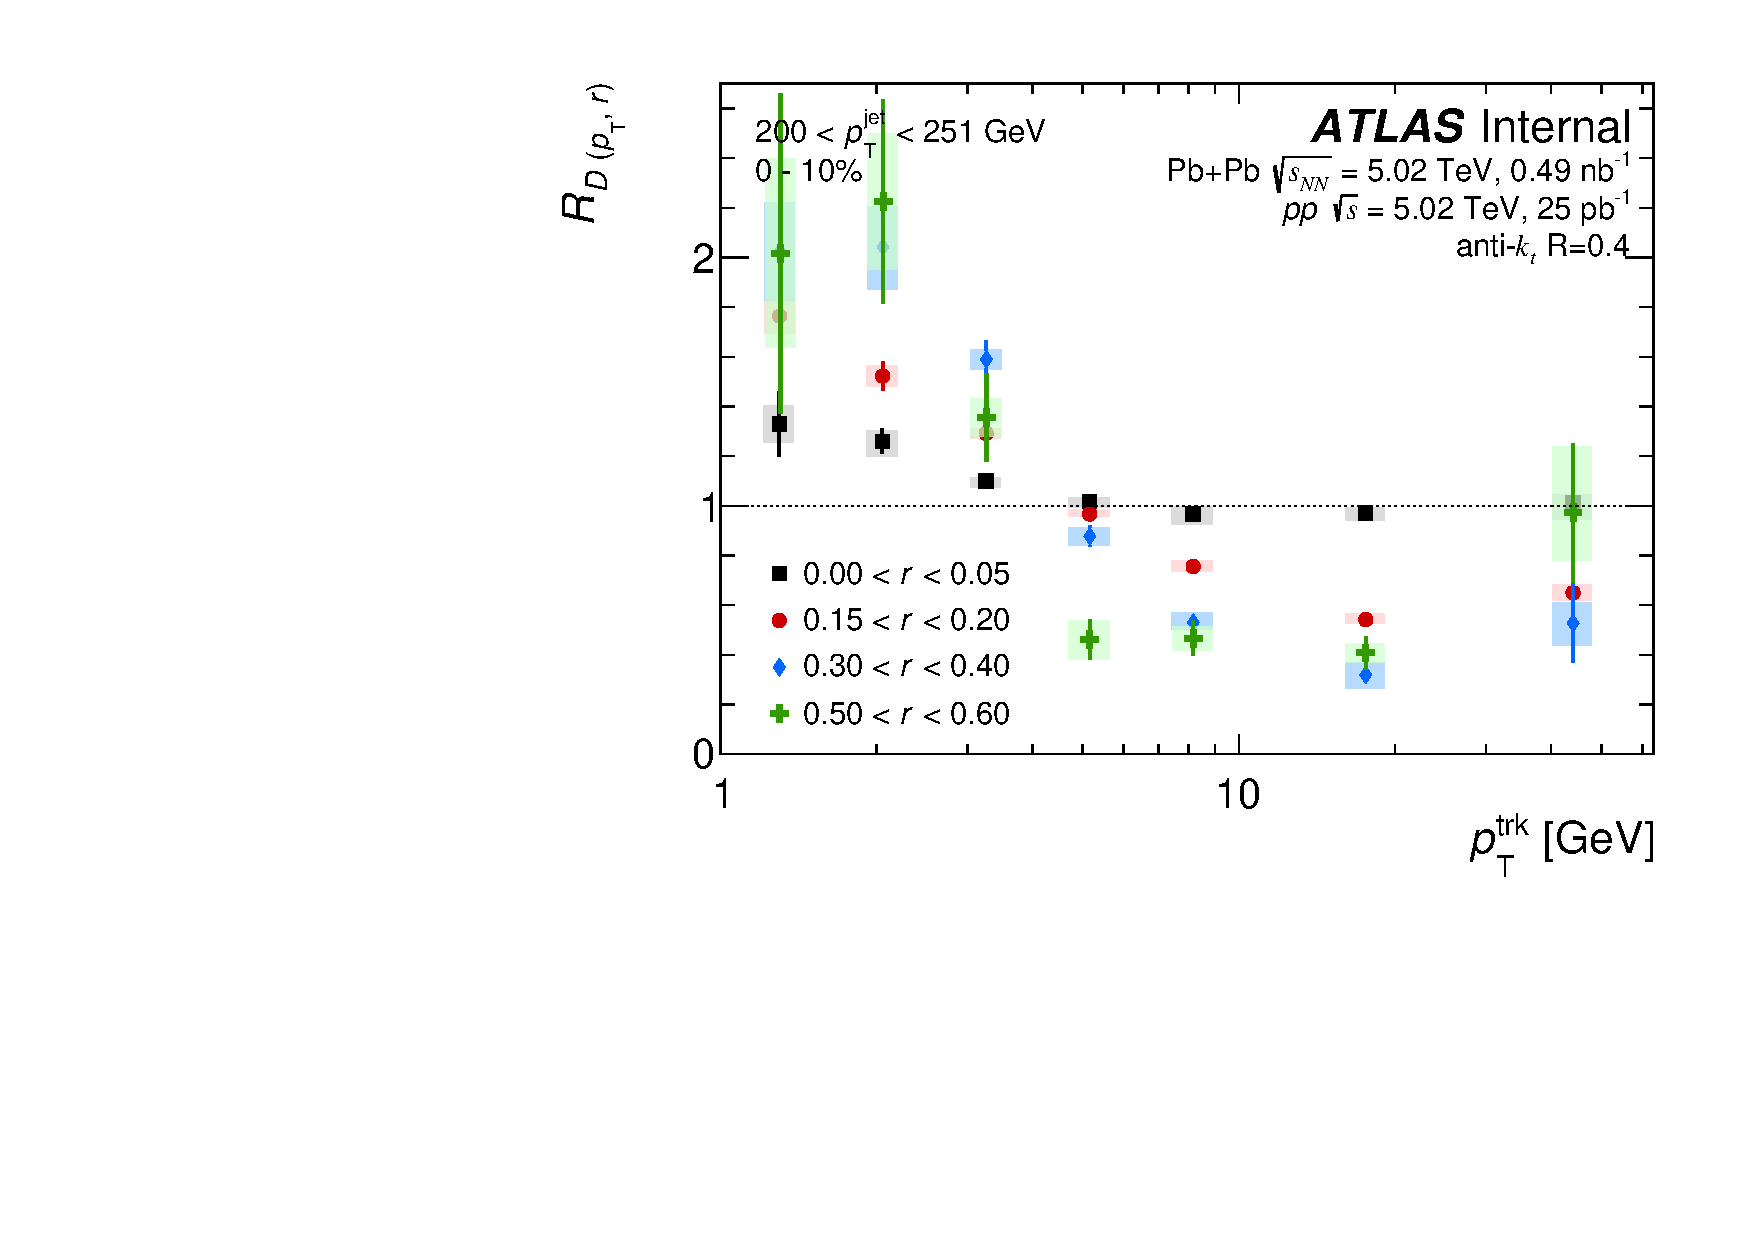
\includegraphics[width=0.45\textwidth]{results/RDpT_final_ratio_dR_CONF_data_trkpT_jet9_cent0} \\
	 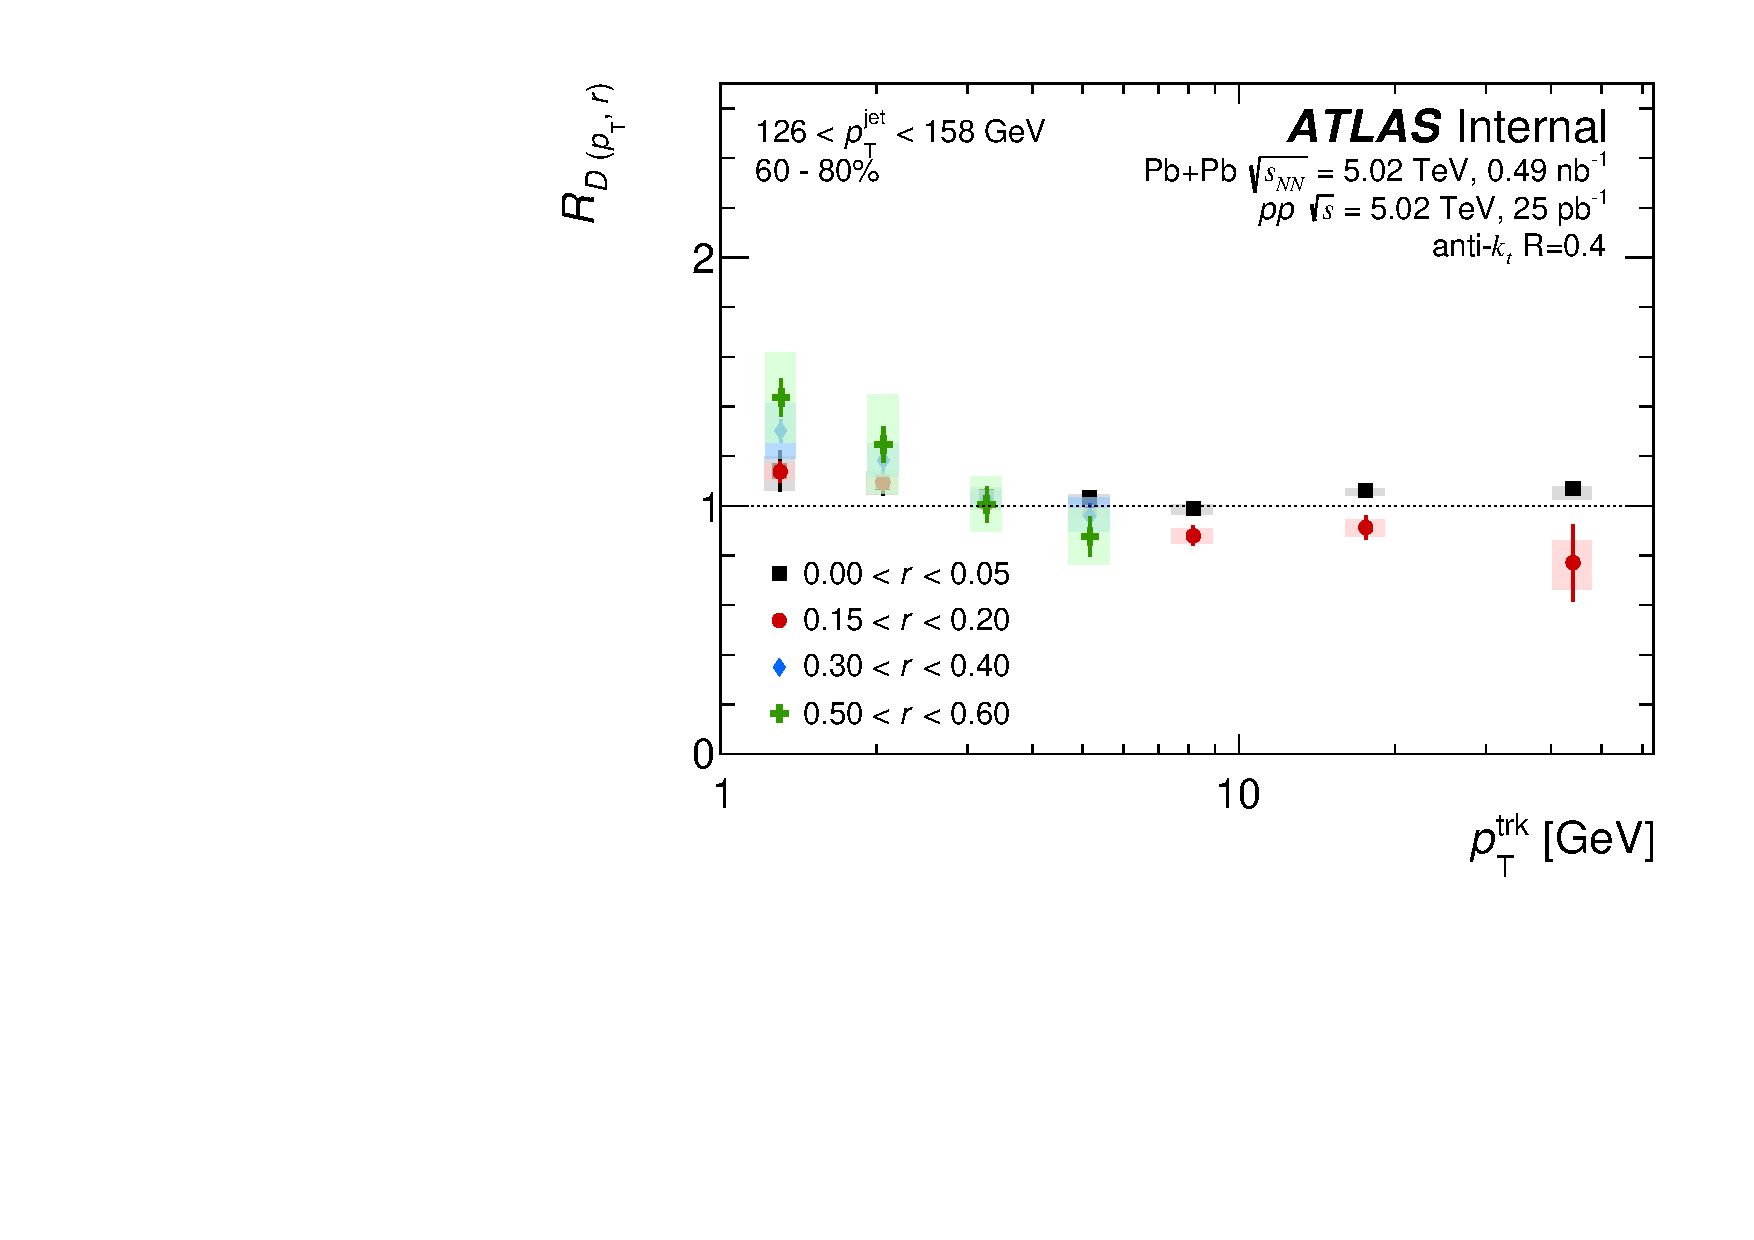
\includegraphics[width=0.45\textwidth]{results/RDpT_final_ratio_dR_CONF_data_trkpT_jet7_cent5} &
	 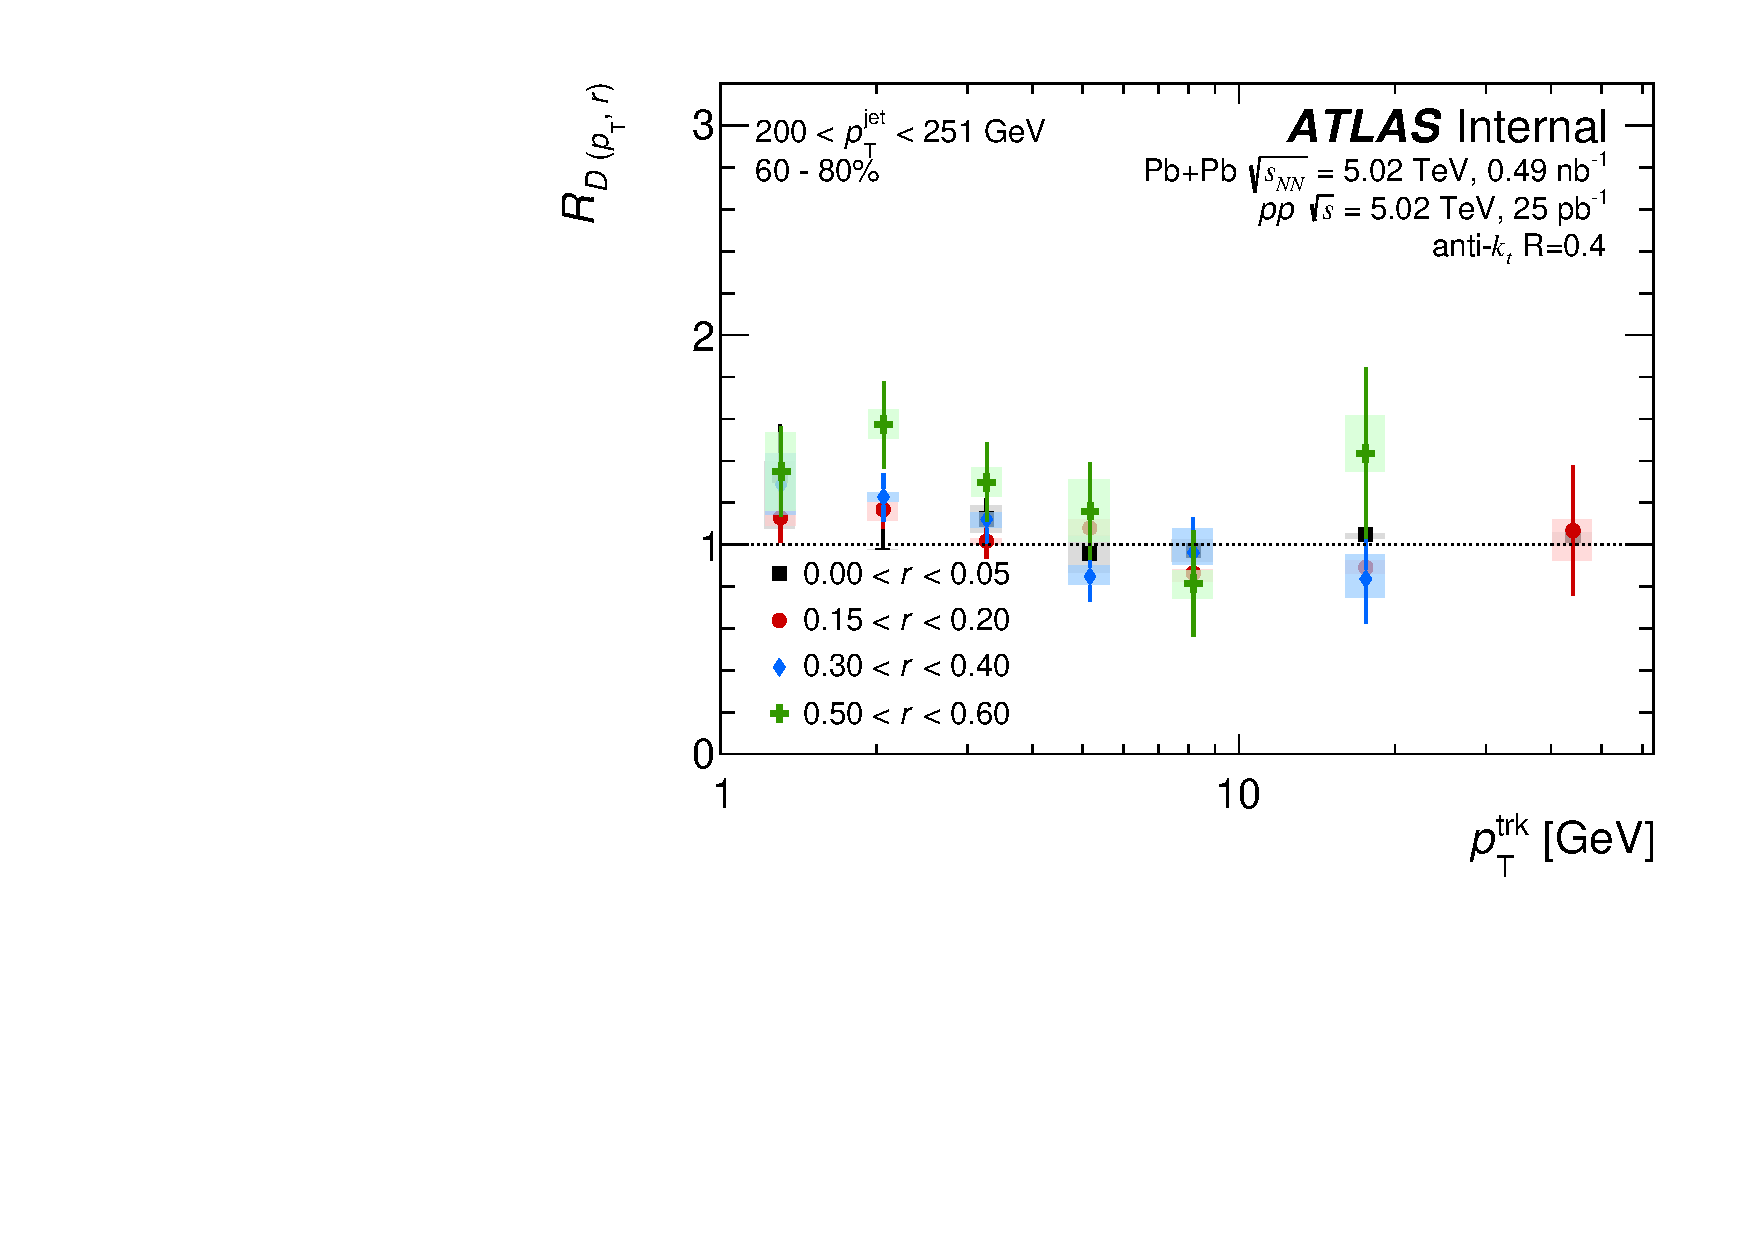
\includegraphics[width=0.45\textwidth]{results/RDpT_final_ratio_dR_CONF_data_trkpT_jet9_cent5} \\
\end{tabular} }
   \caption{\RDptr\ as a function of \pt\ in central (top) and peripheral (bottom) collisions for two different \ptjet\ selections: 126--158~\GeV\ (left) and 200--251~\GeV\ (right). The different colors indicate different distances from the jet axis}
      \label{fig:pttrkdep}
\end{figure}



Differences between the \Dptr\ distributions in \pbpb\ and \pp\ are presented in Figure~\ref{fig:deltadptr} as a function of $r$ for different \pt\ selections. In 0--10\% central collisions. 
These distributions indicate an excess (depletion) in the number of particles in the \pbpb\ system compared to the \pp\ system for low (high) \pt\ particles. This excess ranges from 0.5 to 4 particles for 1 \GeV\ tracks while the depletion ranges from $\sim$0 to 0.5 particles for 10 \GeV\ tracks. An increase in the extra number of particles with increasing \ptjet\ for low \pt\ tracks is also seen.

\begin{figure}
\centering{
\begin{tabular}{cc}
	 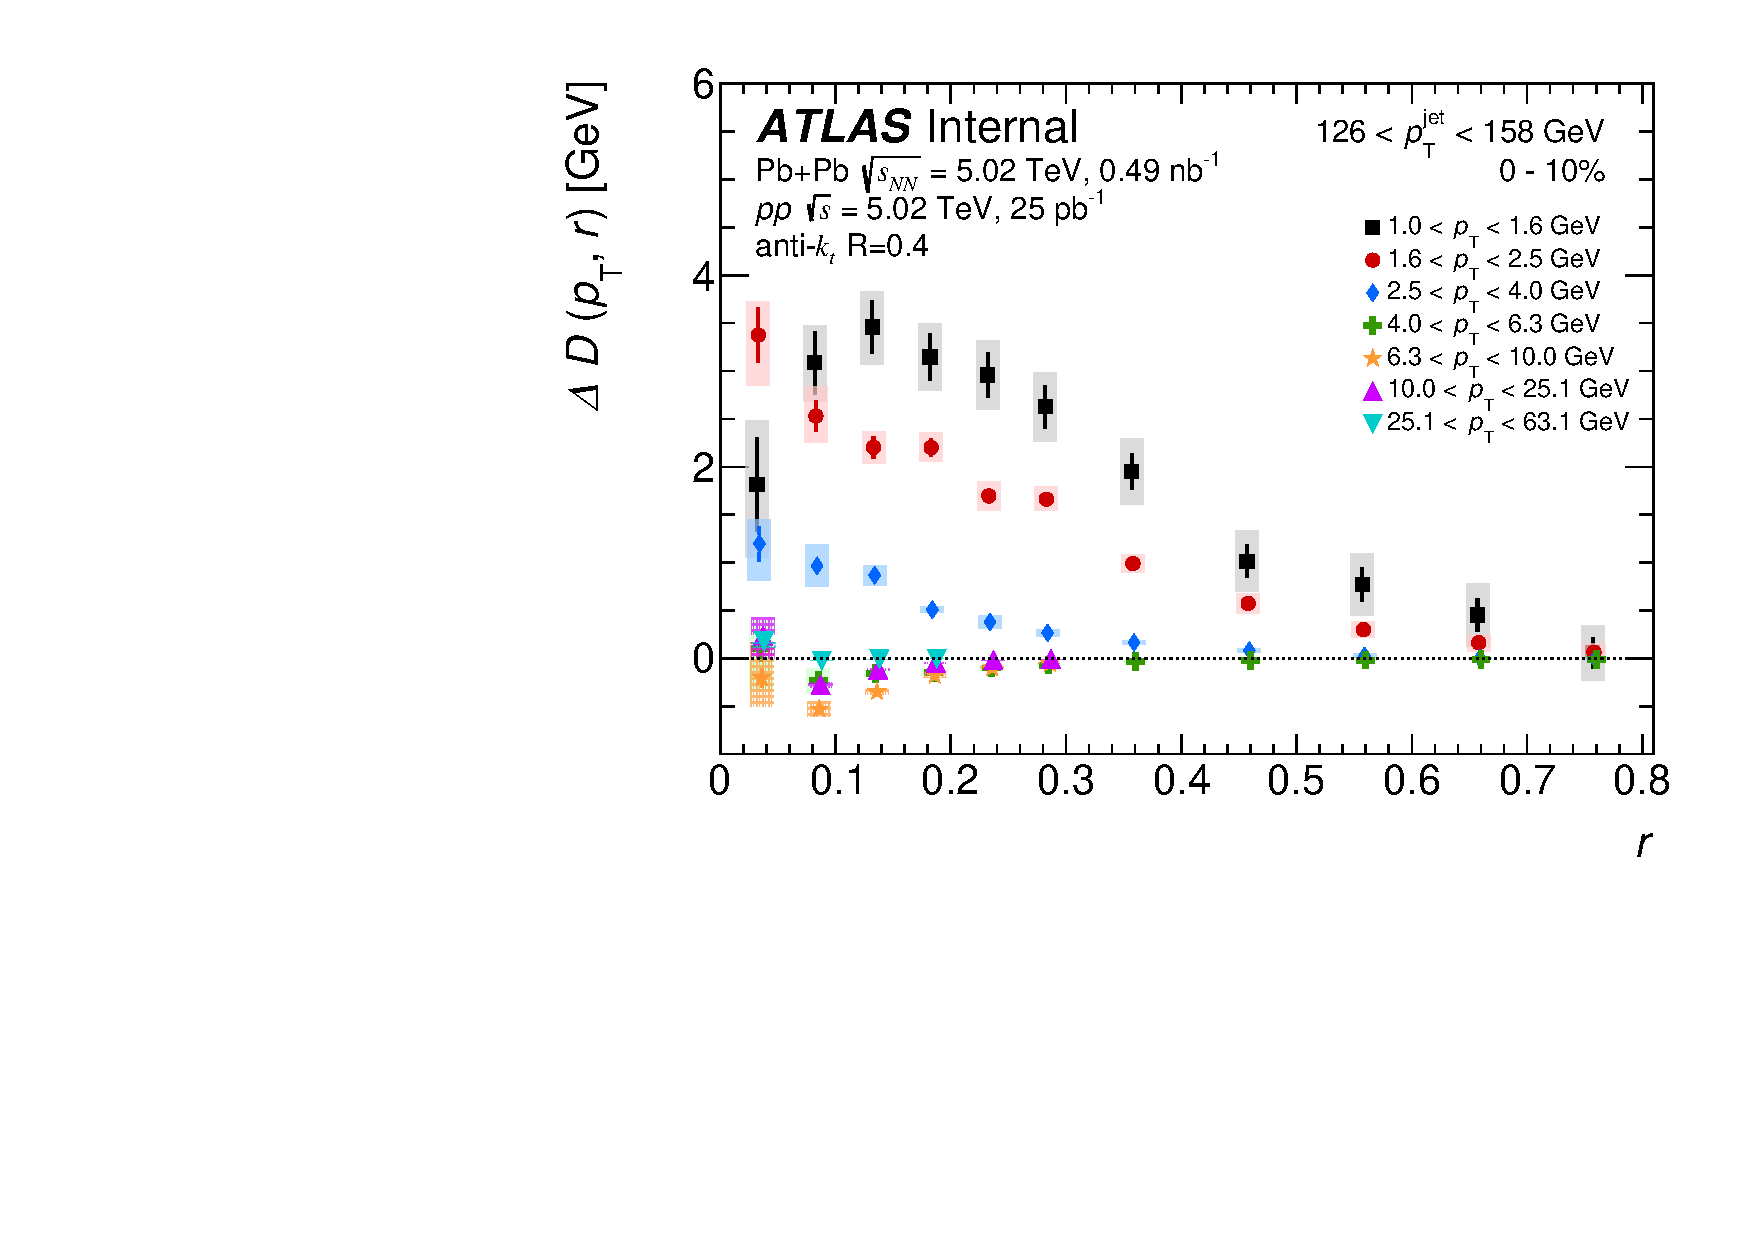
\includegraphics[width=0.45\textwidth]{results/DeltaDpT_final_ratio_dR_CONF_data_jet7_cent0} &
	 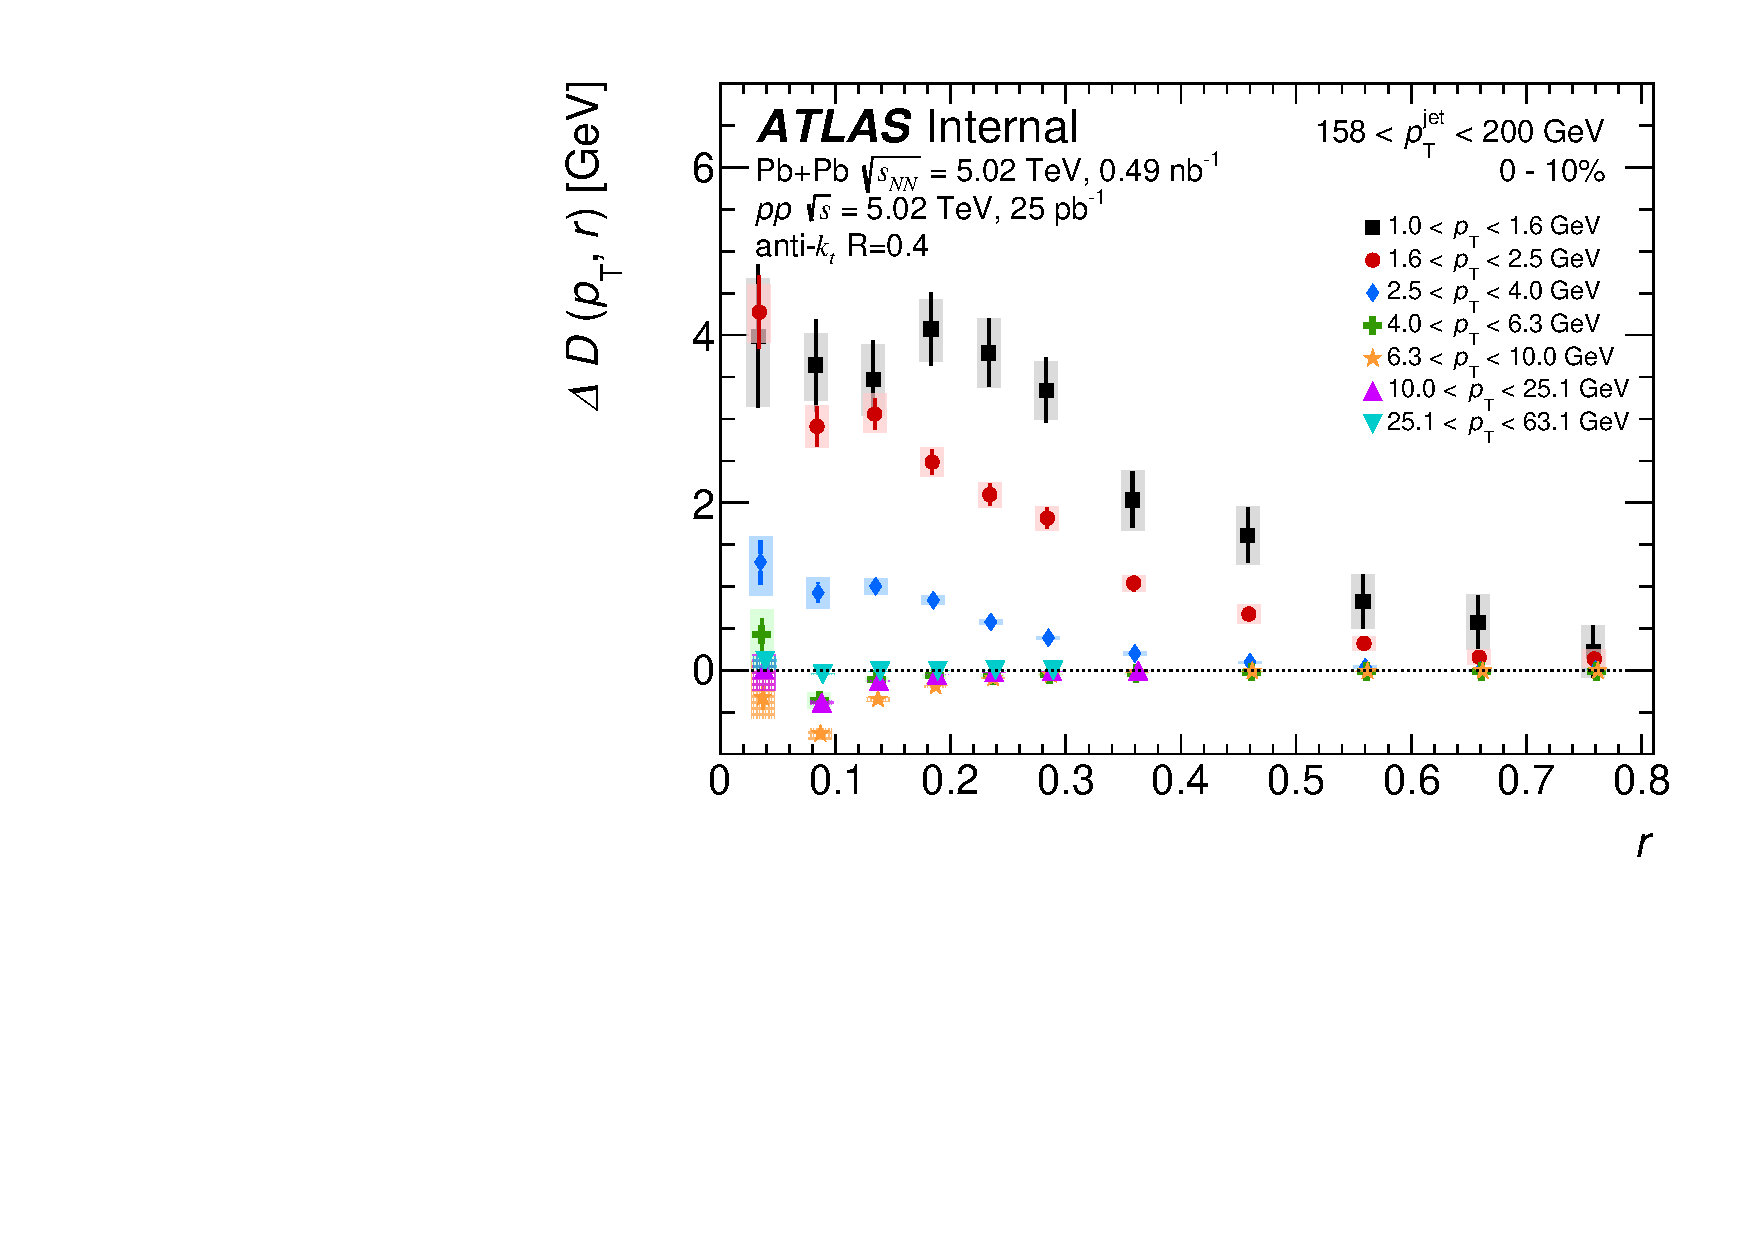
\includegraphics[width=0.45\textwidth]{results/DeltaDpT_final_ratio_dR_CONF_data_jet8_cent0} \\
	 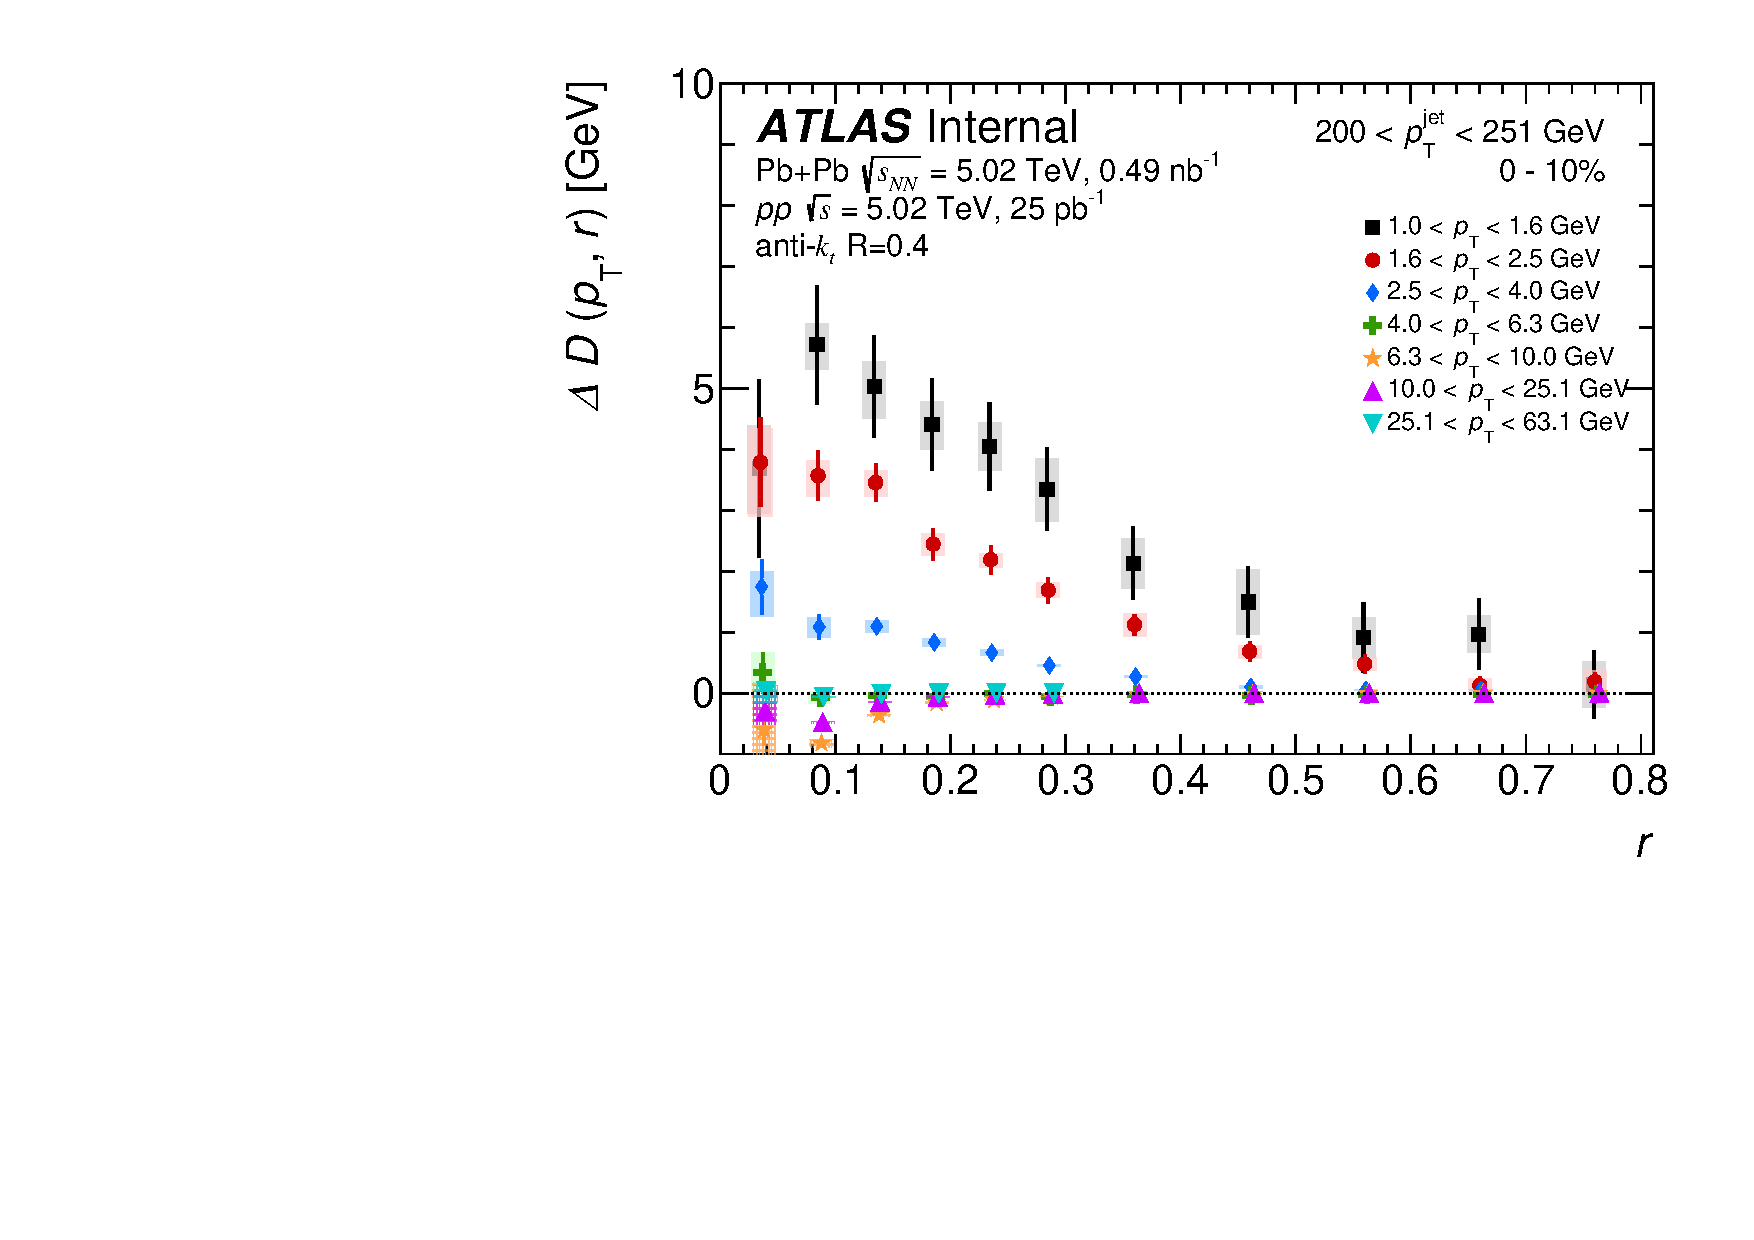
\includegraphics[width=0.45\textwidth]{results/DeltaDpT_final_ratio_dR_CONF_data_jet9_cent0} &
	 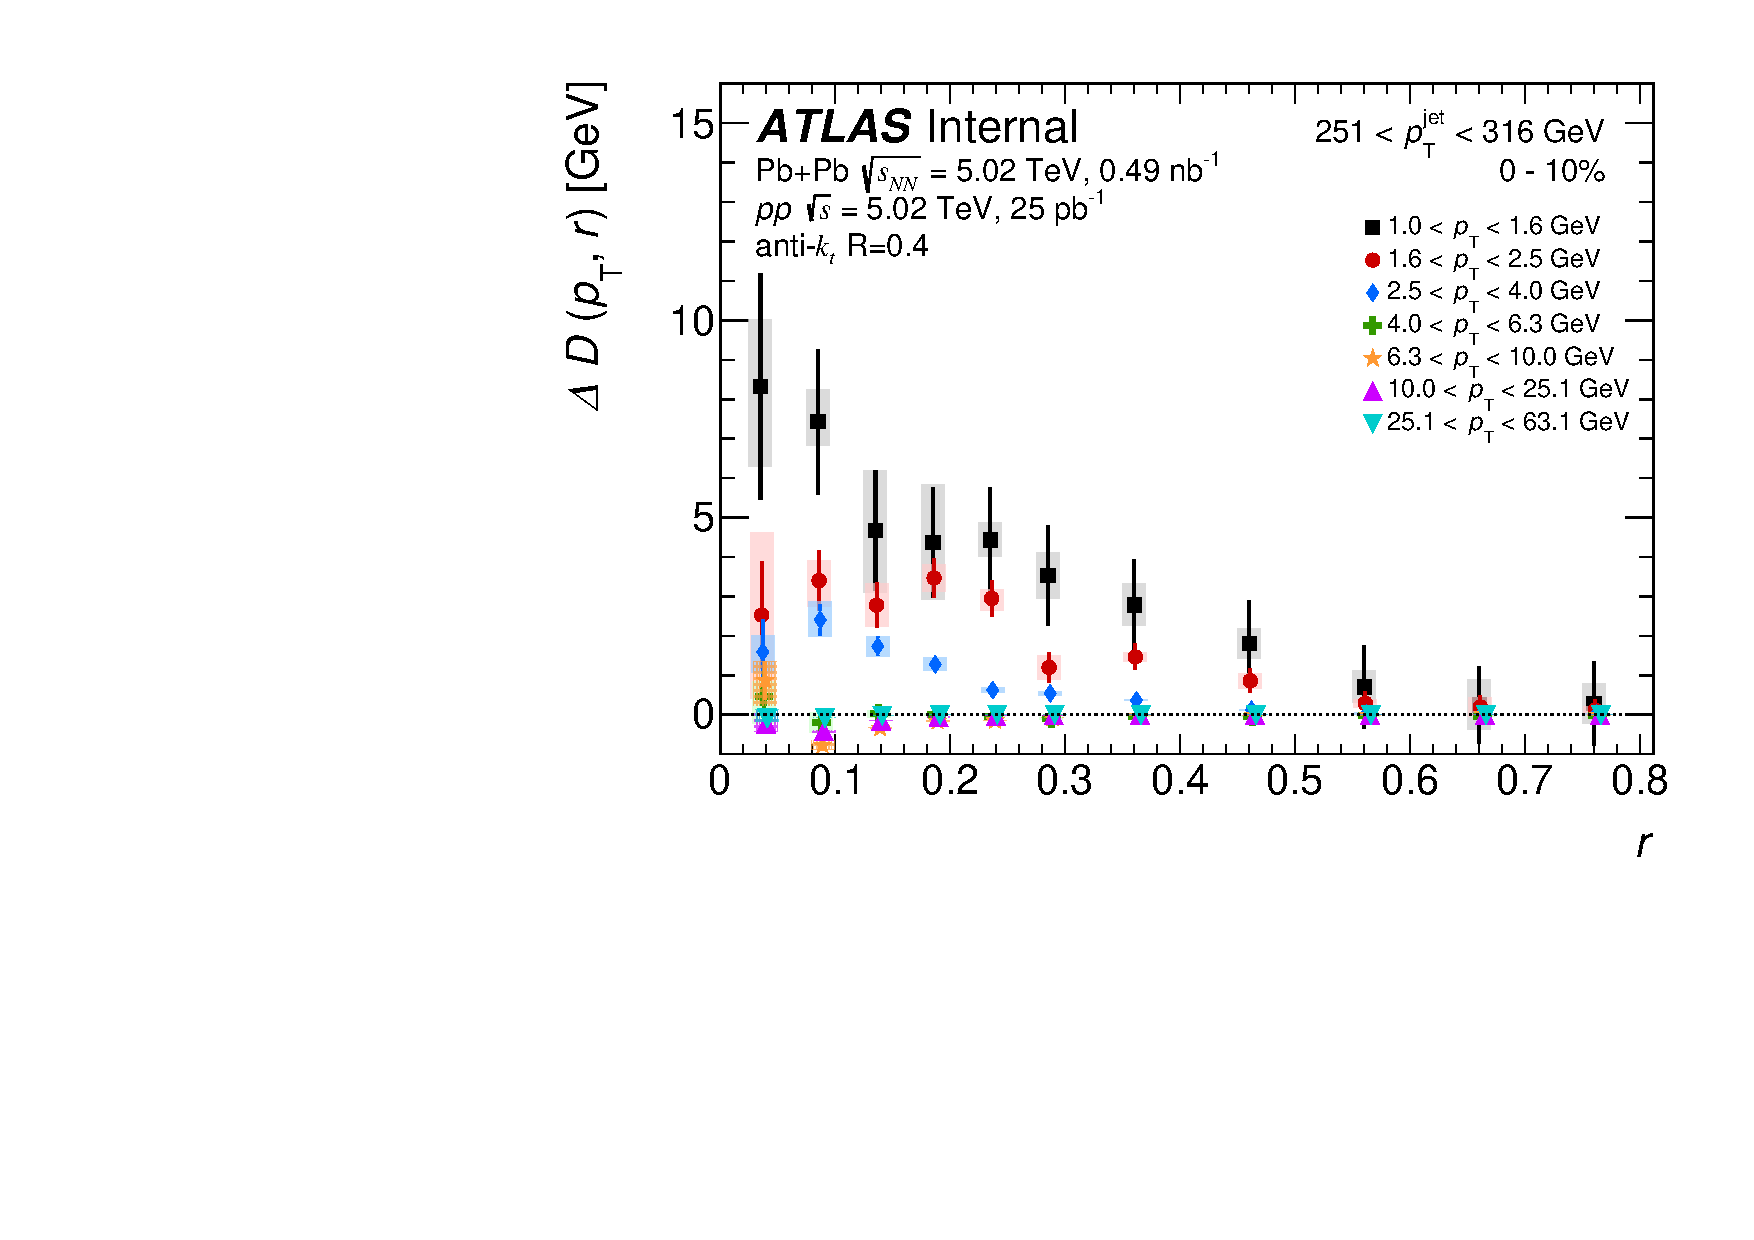
\includegraphics[width=0.45\textwidth]{results/DeltaDpT_final_ratio_dR_CONF_data_jet10_cent0} \\
\end{tabular} }
   \caption{$\Delta \RDptr$ as a function of \rvar\ in central collisions for all \pt\ ranges in four \ptjet\ selections: 126--158~\GeV, 158--200~\GeV, 200--251~\GeV, and 251--316~\GeV. }
      \label{fig:deltadptr}
\end{figure}



\FloatBarrier
